
\chapter{动态MR图像的低秩和稀疏分解模型}
\label{chap:tgvlr}
动态MRI(dynamic MRI, dMRI)是MR成像应用中的一个重要的技术,并且在临床中有着广泛的应用,比如心脏电影成像、磁共振动态对比增强(DCE-MRI)\cite{Yankeelov2009}等,其目的是可视化形态学或者对比度随时间的变化。然而,传统dMRI方法成像速度慢,信噪比低,并且很难在空间分辨率和时间分辨率之间取得平衡 \cite{van1993, Jeffrey2003k, Tsao}。动态MRI重建中最重要的问题是如何平衡时间和空间分辨率,这是由于其数据采集速度慢所决定的。在对动态MR图像进行采样时,如果在每一帧图像上采集了更多的数据,那么在同样的时间内,我们就只能获得更少帧数的数据,造成图像时间分辨率的降低;反之,如果我们保证了时间分辨率,尽可能多的在每一帧图像上都采集数据,那么必然造成在每一帧图像上采集数据的减少,造成空间分辨率的降低。因此,动态MRI的时间分辨率和空间分辨率之间的平衡很难把握。

压缩感知理论\cite{Candes2006Robust}\cite{Donoho2006Compressed}在过去十年中一直是图像处理领域的一个热门话题,并被广泛应用于图像处理领域,尤其是动态MRI\cite{lustig2006,zhaobo,Sajan2011Accelerated,dmrics,kalman,lpluss,han}领域。压缩感知理论证明,我们可以从欠采样的Fourier数据中(通常被称为k-space数据)准确地重建出动态MR图像,这可以显著地减少扫描时间\cite{lustig2006, Lustig2008Compressed}。因此,压缩感知理论可以在加速动态MR成像的同时保证重建图像的时间和空间分辨率。

目前压缩感知在动态MRI\cite{zhaobo,Sajan2011Accelerated,dmrics,kalman,lpluss} 中已经有广泛的应用,我们在小节\ref{sec:cs}中已经有所介绍。这里我们再来回顾一下压缩感知重建动态MR的模型。记动态MR图像为$X\in \mathbb{C}^{N_1\times N_2\times d}$,这里动态图像$X$有$d$帧图像,每帧图像的维度为$N_1\times N_2$。则动态MR成像相过程当于在噪声的干扰下,在k-space中进行动态采样
$$B=AX+\epsilon,$$
其中$A=\mathcal{M}\mathcal{F}$是采样算子,$\mathcal{F}$是作用在每一帧图像上的二维Fourier变换算子,$\mathcal{M}$是作用在每一帧图像上的二维采样模式,$\epsilon$是加性高斯白噪声。于是基于压缩感知的动态MR重建模型可以表示为:
\beq
\min_X \frac{1}{2}\|AX-B\|_{\mathrm{F}}^2+\alpha\|\mathcal{S}X\|_1,
\eeq
其中$\mathcal{S}$是某个稀疏变换,$\alpha$是平衡数据项和稀疏项的参数。

对于动态MR图像而言,稀疏变换$\mathcal{S}$的选择至关重要,而且很具技巧性,主要有以下三种策略。第一种也是最简单的一种是仅仅在模型中利用稀疏项。kt-SPARSE\cite{lustig2006}模型利用了时间和空间上的稀疏项,其模型为:
\beq
\min_X\frac{1}{2}||AX-B||_{\mathrm{F}}^2 + \alpha||\mathcal{W}X||_1 + \beta||\mathcal{F}_tX||_1,
\eeq
其中$\mathcal{W}$是空间方向上的二维小波变换,而$\mathcal{F}_t$是时间上的一维Fourier变换。kt-SPARSE在心脏电影成像中的表现很好,这是因为Fourier变换可以稀疏化周期性运动,比如心脏的搏动。但是,对于其他动态MR图像而言,比如胸部DCE-MRI,胸部组织和肿瘤区域通常不会表现出周期性,因此kt-SPARSE在这类数据中的表现有限。iGrasp\cite{igrasp}结合了压缩感知、平行成像和黄金角度径向采样的思想,提出了只含有一个稀疏约束的模型:
\beq
\min_X\frac{1}{2}||AX-B||_{\mathrm{F}}^2+\alpha||\nabla_t X||_1,
\eeq
其中$\nabla_t$是时间方向的梯度算子。iGrasp在图像时间方向的稀疏性占主导地位时表现很好。但是对于绝大多数动态MR图像来说,空间分辨率和时间分辨率都是十分重要的——高空间分辨率可以帮助医生更好地从视觉上理解图像,而高的时间分辨率在进行图像的量化分析时十分必要。因此仅仅利用时间方向的稀疏项是不足的。

第二种策略是在模型中考虑图像的低秩性,目的是找到一个既稀疏又低秩的解。在这类方法中,动态MR图像通常需要写成二维矩阵形式,矩阵的每一行对应一个像素点,矩阵的每一列对应一帧图像。我们称这种形式的矩阵为Casorati矩阵,其维度为$N_1N_2\times d$。由于动态图像帧与帧之间有着很强的相关性,Casorati矩阵通常可以认为是低秩的。kt-SLR模型不仅利用时间和空间方向的梯度算子,也利用了非凸的Schatten $p$-拟范数。其模型为:
\beq
\min_X \frac{1}{2}\|AX-B\|_{\mathrm{F}}^2+\alpha\|X\|_{\mathrm{3DTV}}+\beta\|X\|_{p}.
\eeq
这里3DTV算子的定义为:
$$
\|\cdot\|_{\mathrm{3DTV}}=\|\nabla_3\cdot\|_1,
$$
而
$$
|\nabla_3\cdot| = \sqrt{(\nabla_x\cdot)^2+(\nabla_y\cdot)^2+\mu(\nabla_t\cdot)^2},
$$
其中$\nabla_x$,$\nabla_y$和$\nabla_t$分别为$x$,$y$和$t$方向上的梯度算子,$\mu$是平衡空间稀疏性与时间稀疏性的参数,$\|\cdot\|_{p}$是Schatten $p$-拟范数,并且$0<p<1$。kt-SLR模型可以提高重建图像的时间分辨率,在心脏灌注图像和体模图像中有良好的表现。但是由于kt-SLR模型使用了TV算子,重建的图像经常会产生阶梯效应。另外,当$0<p<1$时,Schatten $p$-拟范数是非凸的,计算一个稳定的数值解会更加困难。

最后一种策略是利用图像分解的思想,将动态MR图像分解为两个部分的加和,即稀疏部分和低秩部分,并且分别用不同的稀疏项来约束。对于动态图像而言,一方面其背景部分通常随时间变化缓慢,即在时间方向高度相关,这导致了背景部分的低秩性;另一方面其前景部分通常随着时间变化,而且前景部分相对于整幅图像通常比例很小,这导致了前景部分的稀疏性。这样处理的好处是,将背景部分从动态图像中减掉之后,剩下的前景部分会比原图像更加稀疏,因此也更加符合压缩感知理论的条件。Otazo等\cite{lpluss}利用这个想法,提出了L+S模型:
\beq
\min_{L,S}\frac{1}{2}||A(L+S)-B||_\mathrm{F}^2 + \alpha||\nabla_tS||_1 + \beta\|L\|_*,
\eeq
其中$\|\cdot\|_*$为核范数,$L$和$S$分别为低秩部分和稀疏部分。类似的,Trémoulhéac等 \cite{tremoulheac}提出了模型kt-RPCA,其利用时间方向的Fourier变换来约束稀疏部分:
\beq
\min_{L,S}\frac{1}{2}||A(L+S)-B||_\mathrm{F}^2 + \alpha||\mathcal{F}_tS||_1 + \beta\|L\|_*.
\eeq
但是,和模型iGrasp一样,L+S与kt-RPCA也仅仅利用了时间方向的稀疏项。此外,由于模型kt-RPCA中使用了时间方向的Fourier变换,它只在心脏数据中有效果。Schloegl等 \cite{infimaltgv}提出了卷积下确界TGV泛函(infimal convolution TGV,ICTGV),其定义为:
\beq
\mathrm{ICTGV}_{\alpha, \beta}^2(X) = \inf_{X=X_1+X_2}\mathrm{TGV}_{\alpha_1}^2(X_1) + \beta\mathrm{TGV}_{\alpha_2}^2(X_2),
\eeq
相对应的重建模型为:
\beq
\min_{X}\frac{1}{2}||AX-B||_\mathrm{F}^2 + \mathrm{ICTGV}_{\alpha, \beta}^2(X).
\eeq
TGV的概念在文献\cite{bredies2010total}中首次提出,是经典TV的推广。TGV泛函中含有高阶导数项,可以更好地表示图像中的光滑区域,因此可以有效地抑制阶梯效应。虽然模型ICTGV中没有明确地将图像分解为低秩部分和稀疏部分,但是ICTGV可以自适应地将动态图像分解为两个部分,一部分包含更多时间正则项,而另一部分包含更多动态变化。因此我们也将ICTGV归入图像分解的方法。ICTGV可以最优地平衡时间和空间正则项,并且在心脏电影和心脏造影图像上表现良好,但其在胸部DCE-MRI上的表现是未知的。

综上所述,以上针对动态MR图像的压缩感知重建模型要么会导致阶梯效应,要么只利用了时间稀疏项。为了提高重建质量,抑制重建图像中的阶梯效应,并且利用图像分解模型的思想,我们提出了利用二阶时空TGV泛函来约束稀疏部分,利用核范数来约束低秩部分的新模型。具体来说,我们利用核范数来建模时间高度相关的背景,利用二阶时空TGV来刻画背景之上的动态信息。

\section{模型的提出}
\subsection{低秩矩阵补全}
最近几年,低秩矩阵补全算法被广泛应用于动态MR图像重建中。其主要的想法是将动态MR图像看成一个时空矩阵,矩阵的每一行对应动态图像的一个像素点,矩阵的每一列对应动态图像的一帧。在文献\cite{rpca}中,Candès等建立了低秩和稀疏分解模型的数学基础,即鲁棒主成分分析(robust principe component analysis,RPCA)。给定一个Casorati矩阵$X\in \mathbb{C}^{N_1N_2\times d}$,RPCA描述了以下优化问题:
\beq
\min_{L,S} \|L\|_*+\alpha\|S\|_1, \quad s.t.\quad X=L+S.
\label{equ:lpluss}
\eeq
这里核范数作为矩阵的秩的凸松弛,其定义为矩阵奇异值($\sigma_i$)的和:
$$\|\cdot\|_*=\sum_i\sigma_i.$$
Candès指出,在特定的假设下,RPCA可以完美地恢复出低秩和稀疏部分,其中$L$的秩需要很低并且$S$需要有很高的稀疏度。

压缩感知和低秩矩阵填充算法的结合可以进一步加快成像速度,并且将基于图像分解的模型应用于动态MR图像重建是自然而然的:低秩部分可以用来建模时间高度相关的背景,稀疏部分可以建模背景之上的动态信息,如心脏电影图像中心脏的运动和胸部DCE-MRI中造影剂的变化等。目前,已有一些工作\cite{lpluss,tremoulheac}将RPCA的想法应用与动态MR重建中,其中最常用的稀疏变化是时间方向的梯度算子和Fourier变换。

\subsection{二阶时空TGV泛函}
TGV泛函的数学基础由Bredies等\cite{bredies2010total}所建立,是经典TV泛函的推广。TGV泛函可以表示图像中的光滑部分,并且可以在保持图像边缘的同时抑制阶梯效应的产生。因此TGV泛函在很多图像处理问题中都有应用,比如图像去噪\cite{tgv},压缩感知\cite{tgv}等。在本文中,由于所处理的是动态MR图像,我们集中讨论$\mathbb{C}^3$空间中的二阶TGV泛函($\mathrm{TGV}_{\alpha}^2$)。

首先我们回顾$\mathrm{TGV}_{\alpha}^2$的定义。对于$u\in L^1(\Omega), \Omega\subset\mathbb{C}^3$,$\mathrm{TGV}_{\alpha}^2$定义为:
\beq
\begin{aligned}
	\mathrm{TGV}_\alpha^2(u) = &\,\mathrm{sup} \Big\{\int_\Omega u \,\mathrm{div}^2q \,dx \,|\, q\in C_c^2(\Omega,S^{3\times 3}), \\
	&\|q\|_\infty \leq \alpha_0, \|\mathrm{div}\,q\|_\infty \leq \alpha_1 \Big\},
\end{aligned}
\label{equ:tgv}
\eeq
这里$\alpha=(\alpha_0,\alpha_1)$是正参数,$S^{3\times 3}$ 是对称矩阵的集合,$C_c^2({\Omega,S^{3\times 3}})$表示带有紧支撑集且映射到$S^{2\times 2}$的二次连续可微函数。散度算子$\mathrm{div} q\in C_c^1(\Omega, \mathbb{C}^3)$和$\mathrm{div}^2\,q \in C_c(\Omega)$的定义如下:
$$(\mathrm{div}q)_i=\sum^3_{j=1}\frac{\partial q_{ij}}{\partial x_j},$$
$$\mathrm{div}^2q=\sum^3_{j=1}\frac{\partial^2q_{ii}}{\partial x_i^2}+2\sum_{i<j}\frac{\partial q_{ij}}{\partial x_i\partial x_j},$$
其中$q\in C_c(\Omega, S^{3\times 3})$和$p\in C_c(\Omega, \mathbb{C}^3)$的无穷范数为
$$\|q\|_\infty = \sup_{x\in \Omega}(\sum^3_{i=1}|q_{ii}(x)|^2+2\sum_{i<j}|q_{ij}(x)|^2)^{1/2}$$
和
$$\|p\|_\infty = \sup_{x \in \Omega}(\sum_{i=1}^3|p_i(x)|^2)^{1/2}.$$

下面我们回顾一下$\mathrm{TGV}_{\alpha}^2$的基本性质。根据$\mathrm{TGV}_{\alpha}^2$(\ref{equ:tgv})的定义,我们可以得知其空间$L^{p}(\Omega)(1\leq p <\infty)$中是适定的、凸的和下半连续的,并且具有旋转不变性和平移不变性。我们记有界二阶TGV的函数组成的空间为
$$\mathrm{BGV}^2_\alpha(u)=\{u\in L^1(\Omega)|\mathrm{TGV^2_\alpha(u)<\infty}\},$$其范数为
$$\|u\|_{\mathrm{BGV_\alpha^2}}=\|u\|_1+\mathrm{TGV}^2_\alpha(u).$$
我们已知$\mathrm{BGV}^2_\alpha$是一个Banach空间,并且$\mathrm{TGV}_{\alpha}^2$的核空间为:
$$\mathrm{ker}(\mathrm{TGV}^2_\alpha)=\{u(x)=Kx+b \,\big|\, x\in\Omega,K\in \mathbb{C}^2,b\in \mathbb{C}\}.$$
可以看出$\mathrm{TGV}_{\alpha}^2$的核空间由仿射函数组成,所以基于$\mathrm{TGV}_{\alpha}^2$的模型可以很好地估计图像的光滑区域。而TV的核空间由常函数组成,只能估计分片常数的图像,因此基于TV的模型会产生阶梯效应,而基于$\mathrm{TGV}_{\alpha}^2$的模型则不会。

在本文中,我们使用$\mathrm{TGV}_{\alpha}^2$的等价定义:
$$\mathrm{TGV}_\alpha^2(u)=\min_{\omega\in \mathrm{BD}(\Omega)}\alpha_1\|\nabla_3 u-\omega\|_1 + \alpha_0\|\mathcal{E}(\omega)\|_1,$$
其中$\mathcal{E}(\omega)=\frac{1}{2}(\nabla_3\omega+\nabla_3\omega^{T})$是对称梯度算子,$\mathrm{BD}(\Omega)$ 是有界形变函数空间。

\subsection{提出模型}
结合低秩填充和图像分解的思想,我们提出模型:
\beq
\min_{L,S} \frac{1}{2}\|A(L+S)-B\|_{\mathrm{F}}^2+\mathrm{TGV}^2_\alpha(S)+\beta\|L\|_*,
\label{equ:proposed}
\eeq
其中核范数用来建模时间高度相关的背景,二阶时空TGV泛函用来建模背景之上稀疏的动态信息。可以看出,模型是凸的,适定的,并且对于动态MR图像而言是自然而然的。一方面,MR图像通常在梯度域中是稀疏的,而$\mathrm{TGV}_{\alpha}^2$包含了一阶和二阶导数信心,可以很好地稀疏化MR图像。并且从原动态图像中减掉背景之后,剩下的动态信息会比原图像更加稀疏。另一方面,动态图像的背景在时间方向是高度相关的,因此核范数可以完美地建模背景部分。

\section{模型的离散化和算法}
在这一节,我们首先给出$\mathrm{TGV}_{\alpha}^2$的离散格式,然后给出Primal-Dual算法来求解模型的流程。

\subsection{模型离散化}
为了求解模型,我们给出$\mathrm{TGV}_{\alpha}^2$的离散格式。本节的离散化可参照文献\cite{tgv,pd}。首先将区域$\Omega\subset\mathbb{C}^3$离散为网格:
$$\Omega=\{(i,j,k)\big|1\leq i\leq N_1, 1\leq j\leq N_2, 1\leq k\leq d\},$$
其中$N_1$,$N_2$和$d$是动态图像的维度。假设$U=\mathbb{C}^{N_1\times N_2\times d}$, $V=U\times U\times U=U^3$和$W=U\times U\times U\times U\times U\times U=U^6$是三个有限维空间。定义空间$U$中的标量内积$\langle u,u' \rangle _U=\sum_{(i,j,k)\in \Omega}u_{i,j,k}u'_{i,j,k}, u,u'\in U$,范数$\|u\|_U=\sqrt{\langle u,u \rangle _U}$。同样的,$V$和$W$中的标量内积分别为$\langle v,v'\rangle_V=\sum_{i=1}^3\langle v_i,v_i'\rangle_U$和$\langle w,w'\rangle_W=\sum_{i=1}^3\langle w_i,w_i'\rangle_U + 2\sum_{i=4}^6\langle w_i,w_i'\rangle_U$。

在这里,用有限差分来离散$\mathrm{TGV}_{\alpha}^2$,空间步长为1,时间步长由参数$\mu$决定。向前向后差分算子记作:
\begin{align*}
&(\partial_x^+u)_{i,j,k}=\begin{cases}
u_{i+1,j,k}-u_{i,j,k},&1\leq i<N_1,\\
0,&i=N_1,
\end{cases} \\
&(\partial_y^+u)_{i,j,k}=\begin{cases}
u_{i,j+1,k}-u_{i,j,k},&1\leq j<N_2,\\
0, &j=N_2,
\end{cases}\\
&(\partial_t^+u)_{i,j,k}=\begin{cases}
(u_{i,j,k+1}-u_{i,j,k})/\mu,&1\leq k<d,\\
0, &k=d,
\end{cases}\\
\end{align*}
和
\begin{align*}
&(\partial_x^-u)_{i,j,k}=\begin{cases}
u_{1,j,k},&i=1,\\
u_{i,j,k}-u_{i-1,j,k},&1<i<N_1,\\
-u_{m-1,j,k},&i=N_1,
\end{cases}\\
&(\partial_y^-u)_{i,j,k}=\begin{cases}
u_{i,1,k},&j=1,\\
u_{i,j,k}-u_{i,j-1,k},&1<j<N_2,\\
-u_{i,n-1,k},&j=N_2.
\end{cases}\\
&(\partial_t^-u)_{i,j,k}=\begin{cases}
u_{i,j,1}/\mu,&k=1,\\
(u_{i,j,k-1}-u_{i,j,k})/\mu,&1<k<d,\\
-u_{i,j,k-1}/\mu,&k=d.
\end{cases}\\
\end{align*}

梯度算子$\nabla_3$,对称梯度算子$\mathcal{E}$和它们相对应的散度算子为:
\begin{align*}
&\nabla_3: U\rightarrow V,\quad\nabla_3 u =\begin{pmatrix}
\partial_x^+ u\\
\partial_y^+ u\\
\partial_t^+ u\\
\end{pmatrix},  \\
&\mathcal{E}: V\rightarrow W,\quad\mathcal{E} (v) =\begin{pmatrix}
\partial_x^+ v_1\\
\partial_y^+ v_2\\
\partial_t^+ v_3\\
\frac{1}{2}(\partial_y^+ v_1+\partial_x^+ v_2)\\
\frac{1}{2}(\partial_t^+ v_2+\partial_y^+ v_3)\\
\frac{1}{2}(\partial_t^+ v_1+\partial_x^+ v_3)\\
\end{pmatrix},
\end{align*}
和
\begin{align*}
&\text{div}: V\rightarrow U,\quad \text{div}\,v=\partial_x^- v_1+\partial_y^- v_2+\partial_t^- v_3, \\
&\mathrm{div}_2: W\rightarrow V,\quad \mathrm{div}_2\,w=\begin{pmatrix}
\partial_x^- w_1+\partial_y^- w_4+\partial_t^- w_6\\
\partial_x^- w_4+\partial_y^- w_2+\partial_t^- w_5\\
\partial_x^- w_6+\partial_y^- w_5+\partial_t^- w_3\\
\end{pmatrix}.
\end{align*}

由定义,散度算子是梯度算子的复共轭,即$\nabla_3^*=-\text{div}$和$\mathcal{E}^*=-\text{div}_2$。为了定义离散形式的$\mathrm{TGV}_{\alpha}^2$,还需如下的$L^1$和$L^\infty$范数:
\begin{equation*}
\begin{aligned}
u\in U: \quad & \|u\|_1 = \sum_{(i,j,k)\in\Omega} |u_{i,j,k}|, \\
&\|u\|_\infty = \max_{(i,j,k)\in\Omega} |u_{i,j,k}|, \\
v\in V: \quad &\|v\|_1 = \sum_{(i,j,k)\in\Omega}({v_1}_{i,j,k}^2+{v_2}_{i,j,k}^2+{v_3}_{i,j,k}^2)^{1/2}, \\
&\|v\|_\infty = \max_{(i,j,k)\in\Omega}({v_1}_{i,j,k}^2+{v_2}_{i,j,k}^2+{v_3}_{i,j,k}^2)^{1/2},\\
w\in W: \quad &\|w\|_1 = \sum_{(i,j,k)\in\Omega}({w_1}_{i,j,k}^2+{w_2}_{i,j,k}^2+{w_3}_{i,j,k}^2\\&\qquad\qquad\qquad\quad+2{w_4}_{i,j,k}^2+2{w_5}_{i,j,k}^2+2{w_6}_{i,j,k}^2)^{1/2},\\
&\|w\|_\infty = \max_{(i,j,k)\in\Omega}({w_1}_{i,j,k}^2+{w_2}_{i,j,k}^2+{w_3}_{i,j,k}^2\\
&\qquad\qquad\qquad\quad+2{w_4}_{i,j,k}^2+2{w_5}_{i,j,k}^2+2{w_6}_{i,j,k}^2)^{1/2}.
\end{aligned}
\end{equation*}

接下来,我们给出模型(\ref{equ:proposed})的离散格式。假设采样矩阵$A: U \rightarrow Y$,$Y$为有限维度的Hilbert空间,并且为离散形式。则模型(\ref{equ:proposed})可以写成:
\beq
\begin{aligned}
	\min_{(S,w,L)\in U\times V\times U} \alpha_1 \|\nabla_3 S-w\|_1&+\alpha_0\|\mathcal{E}(w)\|_1+\beta\|L\|_*\\
	&+\frac{1}{2}\|A(L+S)-B\|_\mathrm{F}^2,
\end{aligned}
\eeq
其相应的鞍点问题为:
\beq
\begin{aligned}
	\min_{(S,w,L)\in U\times V\times U} &\max_{(p,q,\lambda)\in V\times W\times Y} \langle \nabla_3 S-w,p\rangle+\langle\mathcal{E}(w),q\rangle+\beta\|L\|_* \\
	&+\langle A(L+S)-B,\lambda \rangle-\frac{1}{2}\|\lambda\|_\mathrm{F}^2 \\
	&-\mathcal{I}_{\|\cdot\|_\infty\leq\alpha_1}(p)-\mathcal{I}_{\|\cdot\|_\infty\leq\alpha_0}(q).
\end{aligned}
\label{equ:dual}
\eeq

\subsection{Primal-Dual算法及收敛条件}
在本文中,我们使用Primal-Dual算法\cite{pd}来求解模型。Primal-Dual算法已经被广泛地应用到寻找凸-凹鞍点问题的极大极小问题中:
\beq
\min_{x\in\mathcal{X}}\max_{y\in\mathcal{Y}}\quad\langle \mathcal{K}x,y\rangle+f(x)-g(y),
\label{equ:saddle}
\eeq
其中$\mathcal{X}$和$\mathcal{Y}$是Hilbert空间,$\mathcal{K}:\mathcal{X}\rightarrow\mathcal{Y}$是线性连续映射,并且泛函$f:\mathcal{X}\rightarrow(-\infty,\infty]$和$g:\mathcal{Y}\rightarrow(-\infty,\infty]$是适定的、凸的和下半连续的。为了应用Primal-Dual算法,我们定义预解算子$(I+\tau\partial f)^{-1}$和$(I+\sigma\partial g)^{-1}$,其闭形式的表达分别为:
$$x^*=(I+\tau\partial f)^{-1}(\bar{x})=\argmin_{x\in\mathcal{X}}\frac{\|x-\bar{x}\|_\mathcal{X}^2}{2}+\tau f(x)$$
和
$$y^*=(I+\sigma\partial g)^{-1}(\bar{y})=\argmin_{y\in\mathcal{Y}}\frac{\|y-\bar{y}\|_\mathcal{Y}^2}{2}+\sigma g(y),$$
这里$\tau,\sigma>0$为迭代步长。于是,给定初始点$(x^0,y^0)\in \mathcal{X}\times \mathcal{Y}$并且令$\bar{x}^0=x^0$,Primal-Dual算法有如下迭代步骤:
\beq
\left\{
\begin{aligned}
&y^{n+1}=(I+\sigma\partial g)^{-1}(y^n+\sigma \mathcal{K}\bar{x}^n), \\
&x^{n+1}=(I+\tau\partial f)^{-1}(x^n-\tau \mathcal{K}^*y^{n+1}), \\
&\bar{x}^{x+1}=2x^{n+1}-x^n.
\end{aligned}
\right.
\eeq 
若$\tau\sigma\|\mathcal{K}\|^2<1$,则算法收敛。

接下来,我们将模型(\ref{equ:dual})转化成鞍点问题的结构(\ref{equ:saddle})。令$$\mathcal{X}=U\times V\times U,\quad \mathcal{Y}=V\times W\times Y, \quad
	\mathcal{K}=
\begin{pmatrix}
\nabla_3 & -I & 0\\
0 & \mathcal{E} & 0\\
A & 0 & A
\end{pmatrix},
$$
并且
\begin{equation*}
\begin{aligned}
&f(x)=\beta\|L\|_*,\\
&g(y)=\langle B,\lambda\rangle+\frac{\|\lambda\|_\mathrm{F}^2}{2}+\mathcal{I}_{\|\cdot\|_\infty\leq\alpha_1}(p)+\mathcal{I}_{\|\cdot\|_\infty\leq\alpha_0}(q).
\end{aligned}
\end{equation*}

于是模型(\ref{equ:dual})的求解过程如算法\ref{alg:proposed}的所示。

\begin{algorithm}
	\caption{TGV和低秩分解模型的Primal-Dual算法。}
	\label{alg:proposed}
	\begin{algorithmic}
		\REQUIRE $\sigma$, $\tau$, $S_0$, $L_0$,令 $L_0=A^HB$, $S_0=0$;
		\INDSTATE[-1.25] \textbf{迭代:根据以下步骤更新参数:}	
		\STATE 1. $p^{n+1} = \mathscr{P}_{\alpha_1}(p^n+\sigma(\nabla \bar{S}^n-\bar{w}^n))$;
		\STATE 2. $q^{n+1} = \mathscr{P}_{\alpha_0}(q^n+\sigma\mathcal{E}(\bar{w}^n))$;
		\STATE 3. $\lambda^{n+1} = (\lambda^{n}+\sigma(A(\bar{L}^n+\bar{S}^n)-B))/(1+\sigma)$;
		\STATE 4. $S^{n+1} = S^n-\tau(A^*\lambda^{n+1}-\mathrm{div}_1 p^{n+1})$;
		\STATE 5. $w^{n+1} = w^n+\tau(\mathrm{div}_2q^{n+1}+p^{n+1})$;
		\STATE 6. $L^{n+1} = \mathscr{S}_\beta(L^n-\tau A^*r^{n+1})$;
		\STATE 7. $\bar{S}^{n+1} = 2S^{n+1}-S^n$;
		\STATE 8. $\bar{w}^{n+1} = 2w^{n+1}-w^n$;
		\STATE 9. $\bar{L}^{n+1} = 2L^{n+1}-L^n$;
		\ENSURE $x^{n+1}$。
	\end{algorithmic}
\end{algorithm}

算法步骤中的投影算子$\mathscr{P}_\alpha$为:
$$t^*=\mathscr{P}_\alpha(\bar{t})=\argmin_{\|t\|_\infty\leq \alpha}\frac{\|t-\bar{t}\|^2_\mathrm{F}}{2}=\frac{\bar{t}}{\text{max}(1,\frac{|\bar{t}|}{\alpha})}.$$
收缩算子$\mathscr{S}_\beta$为:
$$t^*=\mathscr{S}_\beta(\bar{t})=\argmin_{t}\frac{\|t-\bar{t}\|_\mathrm{F}^2}{2}+\beta\|t\|_*=\mathrm{U}\mathscr{S}_\beta(\Sigma)\mathrm{V}^T,$$
其中
$$\mathscr{S}_\beta(\Sigma)=\mathrm{diag}\{\text{max}(\sigma_i-\beta,0)\}, i=1,...,r,$$
$\mathrm{U}$,$\Sigma$和$\mathrm{V}$是秩为$r$的矩阵$\bar{t}$的奇异值分解。

为了保证算法收敛性条件$\tau\sigma\|\mathcal{K}\|^2<1$成立,我们需要估计算子$\mathcal{K}$的模。易知$\|\nabla_3\|^2<12$和$\|\mathcal{E}\|^2<12$。记$x=(S,w,L)$,于是
\begin{equation*}
	\begin{aligned}
		\|\mathcal{K}x\|^2&=\|\nabla_3 S-w\|^2+\|\mathcal{E} w\|^2+\|AL+AS\|^2 \\
		& \leq (\|A\|^2+12)\|S\|^2+2\sqrt{12}\|S\|\|w\|+13\|w\|^2\\
		& \ \ \ \ +\|A\|^2\|L\|^2+2\|A\|^2\|S\|\|L\|.
	\end{aligned}
\end{equation*}
因为$2\sqrt{12}\|S\|\|w\|\leq a^2\|S\|^2+12\|w\|^2/a^2, a>0$,并且$2\|A\|^2\|S\|\|L\|\leq \|A\|^2(\|S\|^2+\|L\|^2)$,我们有
\begin{equation*}
	\begin{aligned}
		\|\mathcal{K}x\|^2&\leq(2\|A\|^2+12+a^2)\|S\|^2+(12/a^2+13)\|w\|^2+2\|A\|^2\|L\|^2 \\
		&\leq \mathrm{max}\{2\|A\|^2+12+a^2,12/a^2+13,2\|A\|^2\}\|x\|^2 \\
		& = \mathrm{max}\{2\|A\|^2+12+a^2,12/a^2+13\}\|x\|^2,
	\end{aligned}
\end{equation*}
易知,当$\mathrm{max}\{2\|A\|^2+12+a^2,12/a^2+13\}$取得最小值时,满足$2\|A\|^2+12+a^2=12/a^2+13$,经过计算可得:
$$\|\mathcal{K}\|^2\leq \frac{2\|A\|^2+25+\sqrt{(2\|A\|^2-1)^2+48}}{2}.$$ 

\section{实验设置}
\subsection{实验数据}
我们回顾性地将提出的模型应用在三组不同的动态MR数据集中。第一组数据为生理学改进非均匀心脏躯干数值体模(physiologically improved non uniform cardiac torso,PINCAT),图像维度为$128\times 128\times 50$。第二组数据为活体心脏灌注MR数据(in vivo cardiac perfusion),图像维度为$190\times 90\times 70$ 。这两组数据也被应用在模型kt-SLR中,选择它们是为了更公平地和其他模型进行比较。有关数据集的详细信息,请参考文献\cite{segars2002study, sharif2007adaptive}。

第三组数据是活体胸部DCE-MRI数据。这些数据都来自于不同的病人,并经过了机构审查委员会的批准。这组数据使用了Philips公司的Achieve 3T扫描仪通过破坏性梯度回波序列(spoiled gradient recalled echo, SPGRE)获取,重复时间$T_R$为4.33 ms,回波时间$T_E$为2.12 ms,偏转角为$12^\circ$。采集所得的数据为线圈组合复值数据,维度为$192\times 192\times 10\times 105$,其中相位编码和频率编码均为192,切片数量为10,帧数为105。空间分辨率为$1.33$ mm $\times$ 1.33 mm $\times$ 5 mm,视野大小为256 mm $\times$ 256 mm $\times$ 50 mm。更详细的成像细节请参考文献\cite{li}。我们将这个数据记作Breast1。另外两个胸部数据是在同样的协议不同的成像参数下采集得到的,维度为$192\times 192\times 20\times 25$。我们将这两个数据分别记作Breast2和Breast3。注意,与Breast1不同,Breast2和Breast3只有实值幅度(magnitude)数据。为了缩小论文的焦点,我们只关注通过肿瘤中心的切片。对于Breast1,中心切片为第6个;对于Breast2和Breast3,中心切片为第10个。最终数据的维度分别为$192\times 192\times 105$和$192\times 192\times 25$。

\subsection{比较方法}
我们将提出的模型和最前沿的模型对比,它们分别是kt-SLR\footnote{\url{http://user.engineering.uiowa.edu/~jcb/Software/ktslr_matlab/Software.html}} \cite{Sajan2011Accelerated}, kt-RPCA\footnote{\url{http://agsp.org/bt/ktrpca/}} \cite{tremoulheac}, L+S\footnote{\url{http://cai2r.net/resources/software}} \cite{lpluss} and ICTGV\footnote{\url{https://github.com/IMTtugraz/AVIONIC}} \cite{infimaltgv}。以上模型的程序都使用MATLAB编写,并且全部开源。所有实验程序均在双核Xeon E5-2630 2.2 GHz CPU,128GB内存和NVIDIA TITAN RTX GPU的工作站上运行,MATLAB的版本为2018a。为了加速MATLAB程序,我们也使用CUDA C语言在GPU上实现提出的模型,并且比较了MATLAB和CUDA的运行时间。两个版本的程序均已开源,详细程序请参考网址\url{https://github.com/chixindebaoyu/tgvnn}。

我们选取了两种不同的采样模式进行数值试验,并应用到所有模型中。图\ref{fig:mask3}展示了实验中使用的采样模式,其中图\ref{fig:mask3}(a)是伪径向采样模式。在每一帧图像上,我们均匀地选取一些径向采样线,并使得帧与帧之间的采样线随机转动一个角度以增加非相干性。伪径向采样是动态MR重建数值试验中常用的采样模式,其采样点均在Cartesian网格上,直接使用快速Fourier变换即可实现频率域到图像域的转化,计算快速简便。在所有实验中,如非特别说明,我们均使用32条采样线来保证实验的一致性。伪径向采样的总加速因子为6.6,这里的总加速因子为k-space中所有点的个数与k-space采样点个数的比值。为了测试提出的模型在不同采样模式下的表现,我们也选取了Cartesian采样模式进行试验,如图\ref{fig:mask3}(b)所示。Cartesian采样模式是临床MR成像最常用的采样模式。在每一帧图像上,我们对低频区域进行全采样,对高频区域进行随进采样。具体来说,我们在k-space中选取中心窗口大小为20的区域作为低频区域,而在外围的高频区域,我们随机选择一些相位编码线来增加非相干性,使得总体来说外围的每一条相位编码线被选取的次数相同,并且帧与帧之间达到最大的正交性。Cartesian采样的总加速因子为5.1。
\begin{figure}[htbp]
\centering
\subfigure[动态伪随机采样(一帧)]{
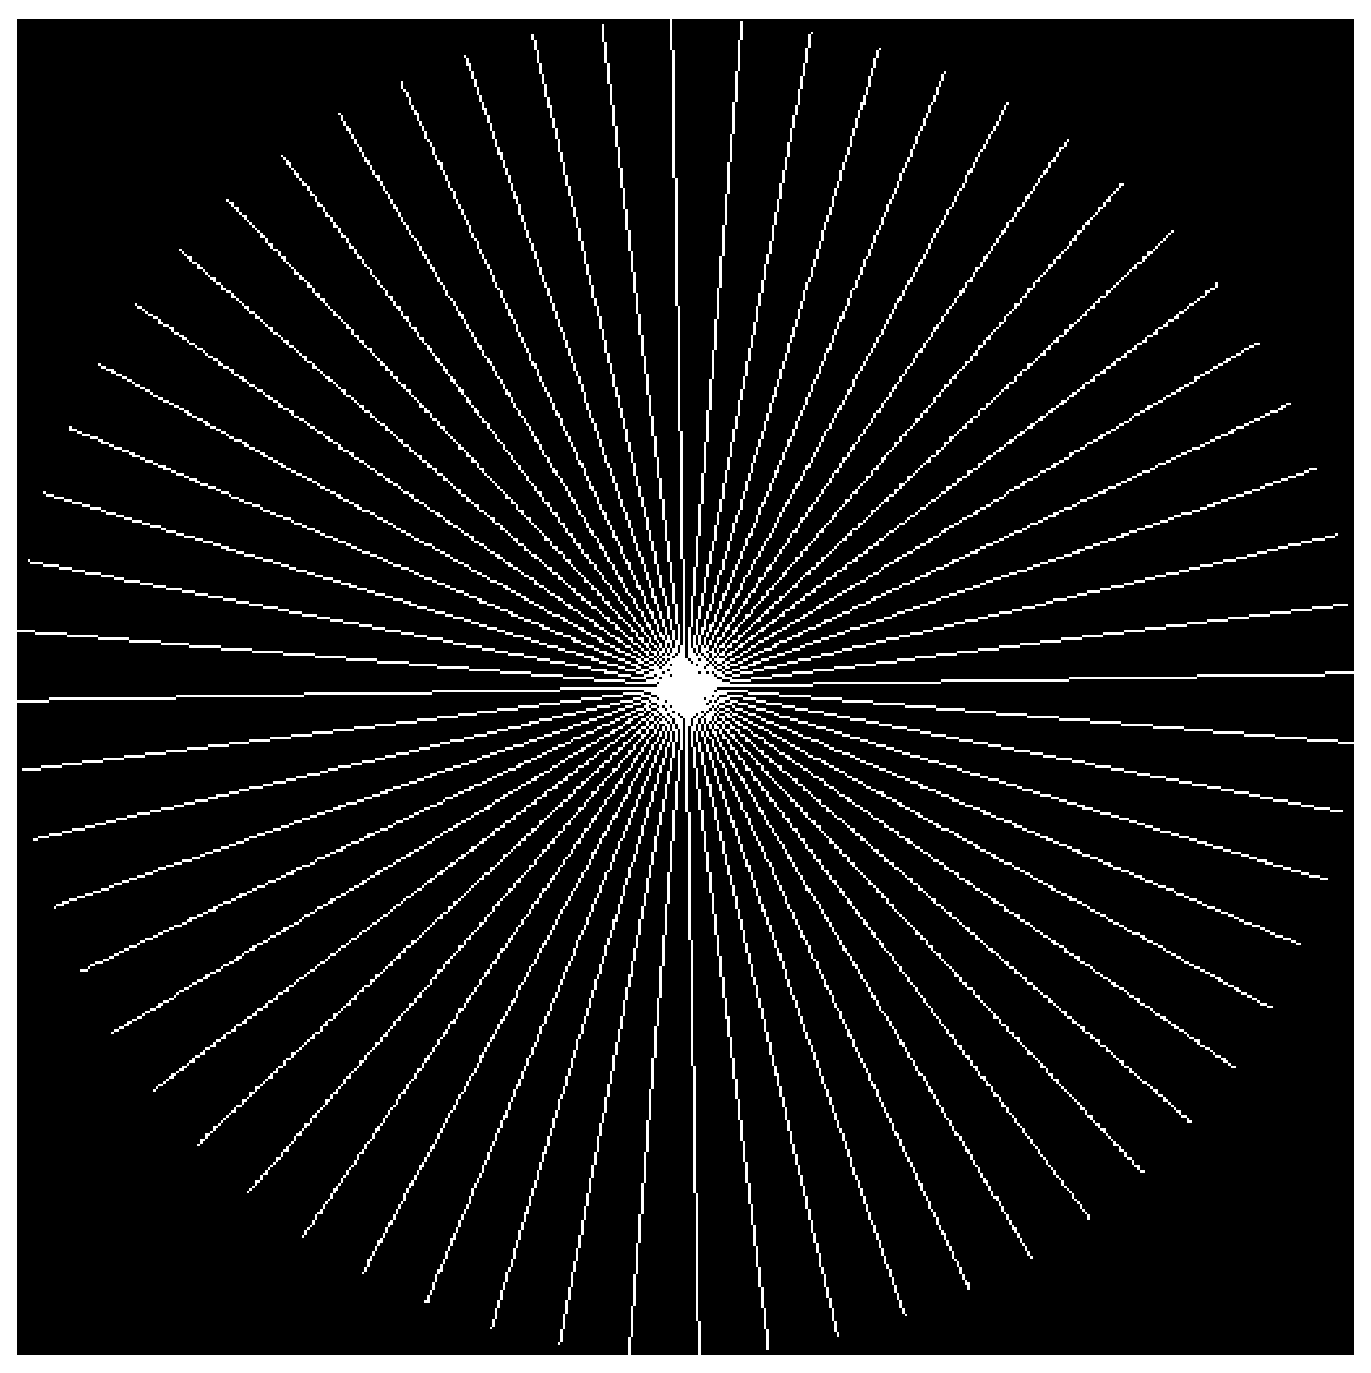
\includegraphics[width=2.5in]{img/intro/pradial.eps}
}
\subfigure[动态Cartesian采样(一帧)]{
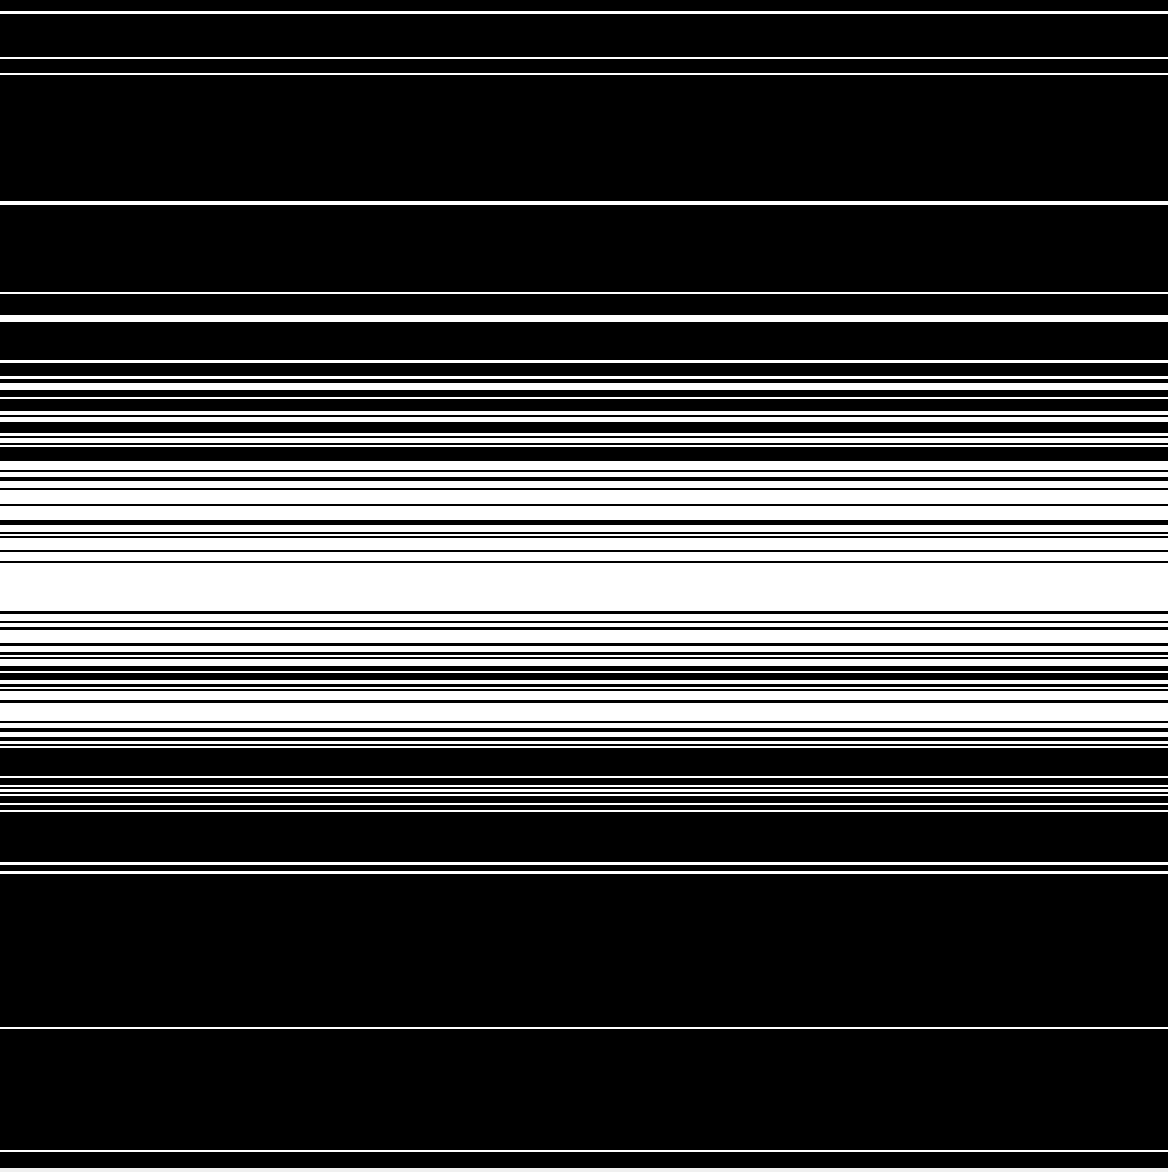
\includegraphics[width=2.5in]{img/intro/cartesian.png}
}
\centering
\caption{文章使用的动态采样模式(一帧)。}
\label{fig:mask3}
\end{figure}

实验使用的评估方法为信噪比(signal error ratio,SER)和相似性测度\cite{ssim}(structural similarity index,SSIM),它们是压缩感知重建中最常用到的评估方法。SER的定义为:
$$\mathrm{SER} = -10\log_{10}\frac{\|X_\mathrm{rec}-X_\mathrm{ori}\|_\mathrm{F}^2}{\|X_\mathrm{ori}\|_\mathrm{F}^2},$$
其中$X_\mathrm{rec}$为重建后的图像,$X_\mathrm{ori}$为原始的、全采样图像。SSIM的定义为
$$\mathrm{SSIM} = \frac{(2\mu_\mathrm{rec}\mu_\mathrm{ori}+c_1)(2\sigma_{\mathrm{rec},\mathrm{ori}}+c_2)}{(\mu_\mathrm{rec}^2+\mu_\mathrm{ori}^2+c_1)(\sigma_\mathrm{rec}^2+\sigma_\mathrm{ori}^2+c_2)},$$
其中$\mu_\mathrm{ori}$和$\mu_\mathrm{rec}$分别为原始图像和重建图像的均值,$\sigma_\mathrm{ori}$和$\sigma_\mathrm{rec}$分别为原始图像和重建图像的方差,$\sigma_{\mathrm{rec,ori}}$为原始图像和重建图像之间的协方差,$c_1$和$c_2$为常数。由于我们处理的是动态MR图像,这里的SSIM计算为每一帧的平均值。实验时为了保证一致性,所有数据都被缩放到[0,1]。我们通过以下方法调试模型参数:对于PINCAT数据,通过对每个参数进行穷举搜索得到最高SER时的参数,并将此参数用于其他数据集中。表\ref{tab:params}展示了提出模型所使用的参数。为了保证算法收敛,伪径向采样的迭代次数设置为500,Cartesian采样的迭代次数设置为1000。
\begin{table}[htbp]
	\centering
	\caption{文章提出模型使用的参数}
	\begin{tabular}{|c|c|c|c|c|c|c|c|}
		\hline
		\hline
		\diagbox{采样模式}{参数}& $\alpha_0$ & $\alpha_1$ & $\beta$ & $\sigma$ & $\tau$ & $\mu$ & iter\\	
		\hline
		Pseudo radial & 0.006 & 0.004 & 0.5 & 0.25 & 0.25 & 1 & 500\\
		\hline
		Cartesian & 0.015 & 0.005 & 0.08 & 0.28 & 0.28 & 1 & 1500\\
		\hline
	\end{tabular}
	\label{tab:params}
\end{table}

\section{实验结果}
表\ref{tab:result3}展示了在伪径向采样模式下,各个模型在不同数据上重建结果的比较。可以看出本文的模型在所有的数据集上都取得了很好地效果,尤其是在cardiac和胸部DCE-MRI数据上,SER和SSIM均为最高。虽然kt-SLR在PINCAT数据上的SER最高,其在胸部数据上的表现很差。同样的,kt-RPCA虽然在胸部数据上的表现仅次于本文提出的模型,但其在PINCAT和cardiac数据上的表现一般。
\begin{table}
	\centering
	\caption{各个模型在不同数据上的重建结果}
	\begin{tabular}{|c|c|c|c|c|c|c|}
		\hline
		\hline
		\multicolumn{2}{|c|}{\diagbox{模型}{数据集}}& PINCAT & cardiac & Breast1 & Breast2 & Breast3\\	
		\hline
		\multirow{2}{*}{Zerofilled}
		&SER & 20.54 & 14.80 & 11.32 & 11.57 & 14.85\\
		\cline{2-7}&SSIM & 0.8321 & 0.8855 & 0.4820 & 0.5897 & 0.7086\\
		\hline
		\multirow{2}{*}{kt-SLR}
		&SER & \textbf{33.35} & 17.58 & 17.42 & 13.61 & 18.38\\
		\cline{2-7}&SSIM & 0.9880 & 0.9412 & 0.7712 & 0.6956 & 0.8461\\
		\hline
		\multirow{2}{*}{kt-RPCA}
		&SER & 29.27 & 18.33 & 19.31 & 14.82 & 19.81\\
		\cline{2-7}&SSIM & 0.9700 & 0.9447 & 0.8857 & 0.7920 & 0.9068\\
		\hline
		\multirow{2}{*}{L+S}
		&SER & 27.99 & 19.12 & 17.60 & 14.74 & 19.91\\
		\cline{2-7}&SSIM & 0.9514 & 0.9490 & 0.7675 & 0.7319 & 0.8791\\
		\hline
		\multirow{2}{*}{ICTGV}
		&SER & 26.88 & 17.87 & 16.31 & 12.18 & 16.84\\
		\cline{2-7}&SSIM & 0.9435 & 0.9405 & 0.6735 & 0.6080 & 0.7693\\
		\hline
		\multirow{2}{*}{Proposed}
		&SER & 32.74 & \textbf{19.57} & \textbf{20.56} & \textbf{16.24} & \textbf{21.08}\\
		\cline{2-7}&SSIM & \textbf{0.9917} & \textbf{0.9514} & \textbf{0.9402} & \textbf{0.9091} & \textbf{0.9356}\\
		\hline
	\end{tabular}
	\label{tab:result3}
\end{table}

图\ref{fig:pincat}展示了各个模型在PINCAT数据上第1帧的重建结果。重点看红色箭头,虽然kt-SLR取得了最高的SER(33.35),其重建的图像中仍然残留有空间伪影,而本文提出的方法中则没有。此外,蓝色箭头表明本文的方法在保持边缘和抑制伪影方面的表现要优于kt-RPCA,L+S和ICTGV。
\begin{figure}
\centering
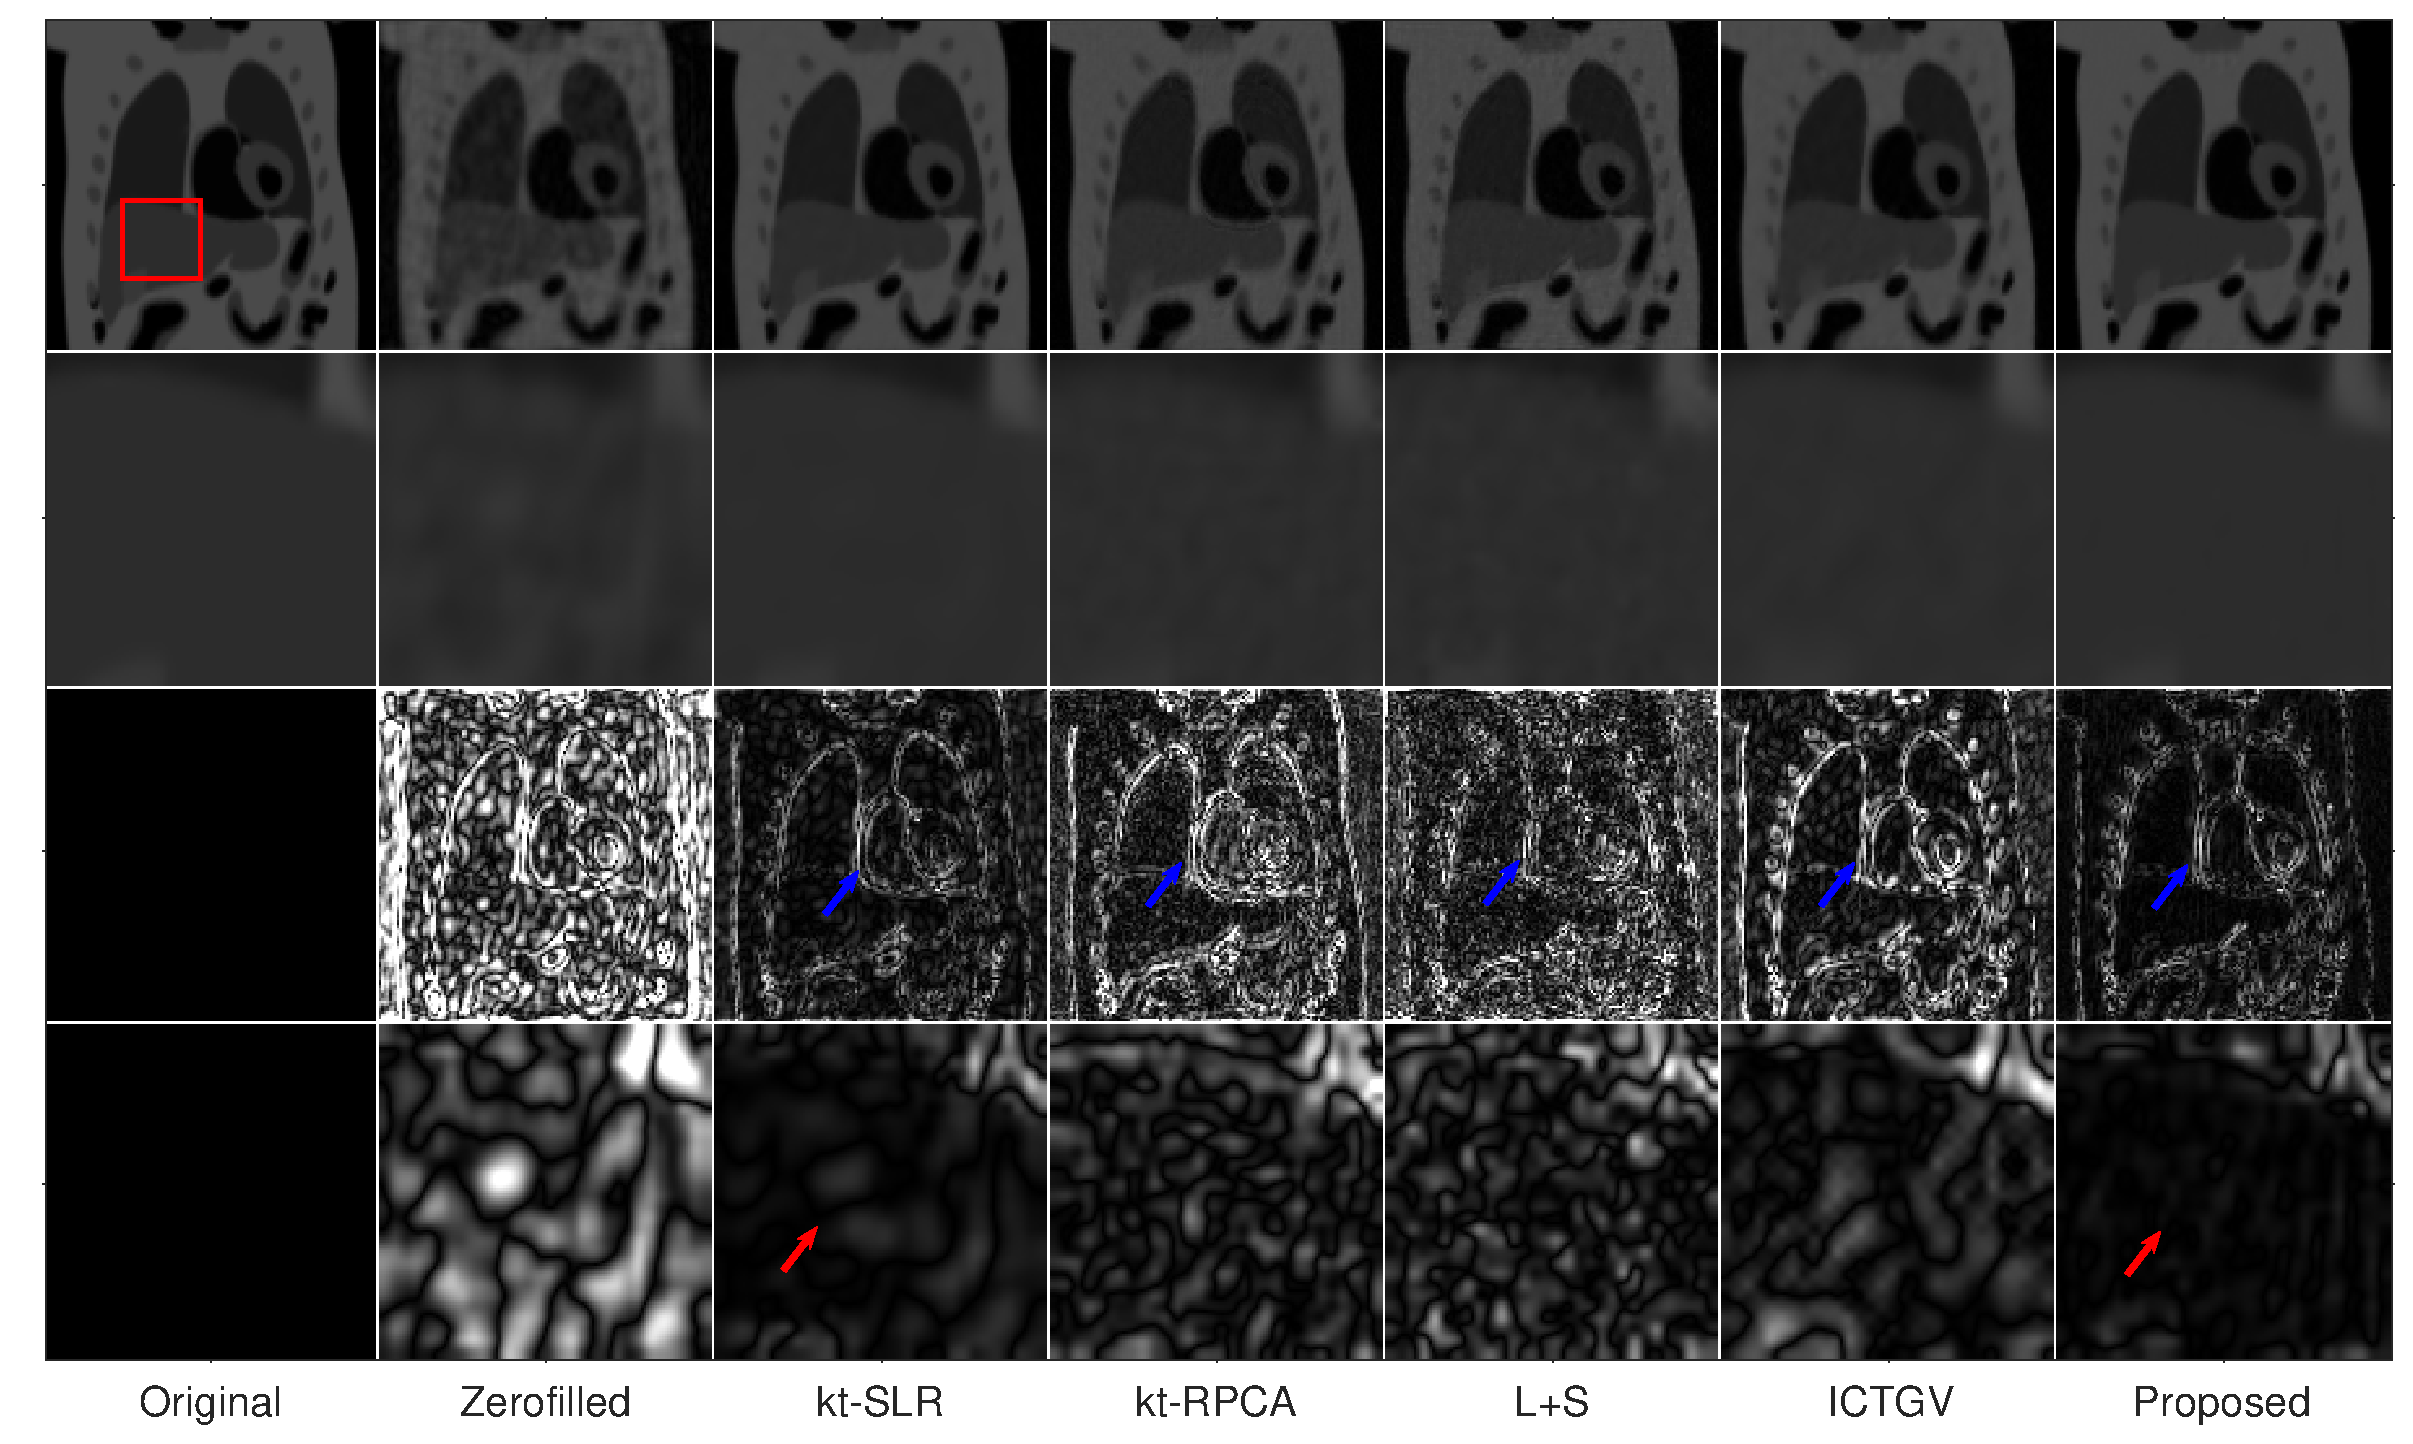
\includegraphics[width=1\textwidth]{img/tgvnn/figure2_pincat.eps}
\caption{各个模型在PINCAT数据上的重建结果(第1帧)。第1行:重建图像;第2行:红色方框区域的放大图像;第3行:相对于原始图像的差值图像;第4行:红色方框区域放大的差值图像。为了增加可见度,差值图像放大了30倍。}
\label{fig:pincat}
\end{figure}

图\ref{fig:pincat}展示了各个模型在心脏灌注数据上第1帧的重建结果。本文的模型取得了最高的SER(19.58)和SSIM(0.9514),并且重建图像中的伪影最少。红色箭头表明kt-SLR,kt-RPCA和ICTGV的表现很差,尤其在保持图像边缘上。虽然L+S在心脏灌注数据上的表现很好,蓝色箭头表明本文模型的重建图像比L+S更加光滑。
\begin{figure}
\centering
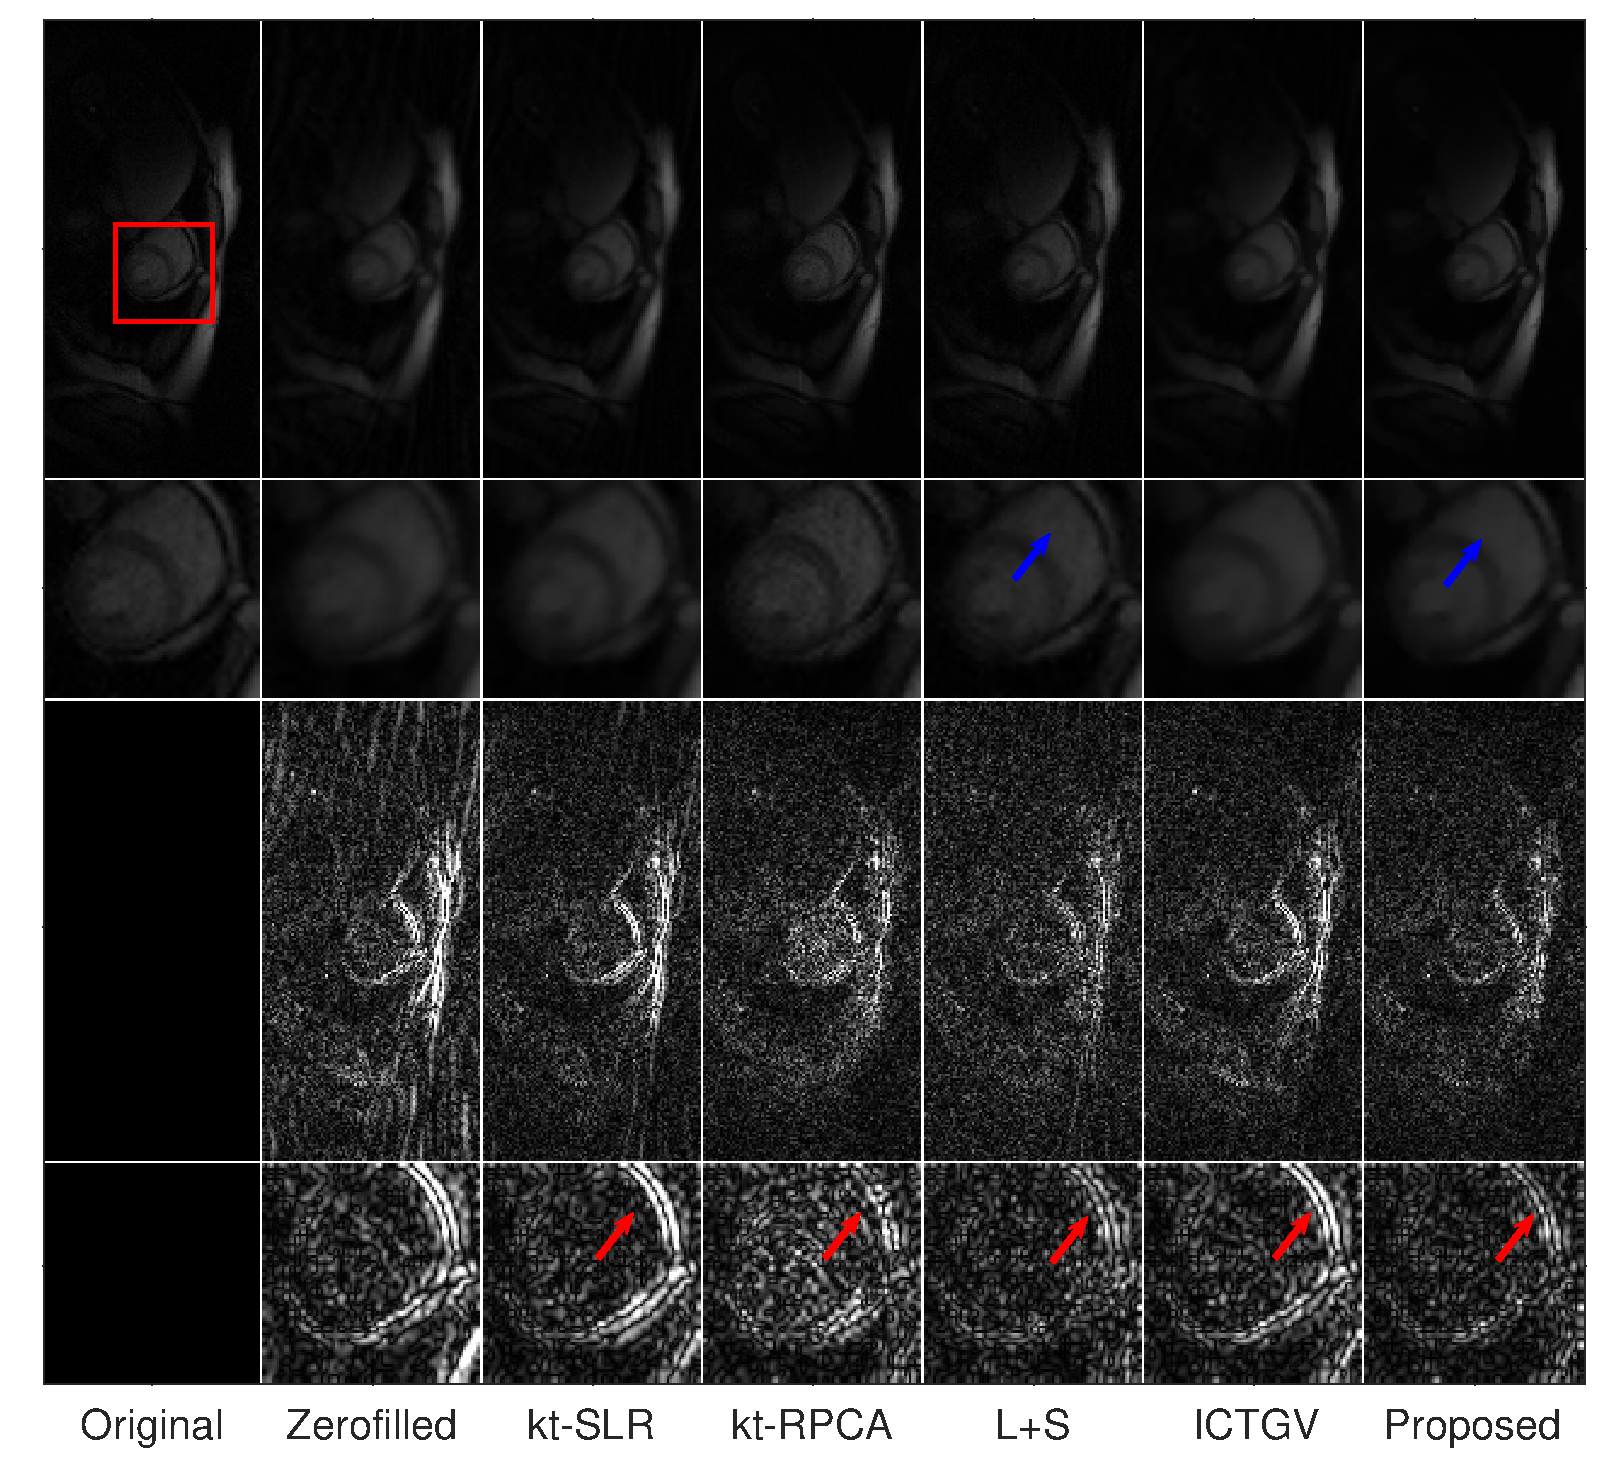
\includegraphics[width=1\textwidth]{img/tgvnn/figure3_perfusion.eps}
\caption{各个模型在cardiac数据上的重建结果(第1帧)。第1行:重建图像;第2行:红色方框区域的放大图像;第3行:相对于原始图像的差值图像;第4行:红色方框区域放大的差值图像。为了增加可见度,差值图像放大了20倍。}
\label{fig:perfusion}
\end{figure}

为了比较时间方向上的重建效果,我们针对心脏灌注数据展示了各个模型不同帧与时间序列图像的结果,如图\ref{fig:perfusion_frames}所示。可以看到,本文的模型的重建图像在视觉上的质量最高。红色箭头显示出kt-SLR的重建图像很模糊,这导致了低SER。蓝色箭头表明kt-RPCA的重建图像有严重的运动伪影,尤其在心脏的边缘部分。同时我们也可以从黄色箭头看出,kt-RPCA和ICTGV在时间上有过平滑效应,尤其是ICTGV。L+S在SER和时间序列图像上的表现很好,但是由于L+S没有空间方向的约束,其重建图像的每一帧都有噪声(绿色箭头)。
\begin{figure}
\centering
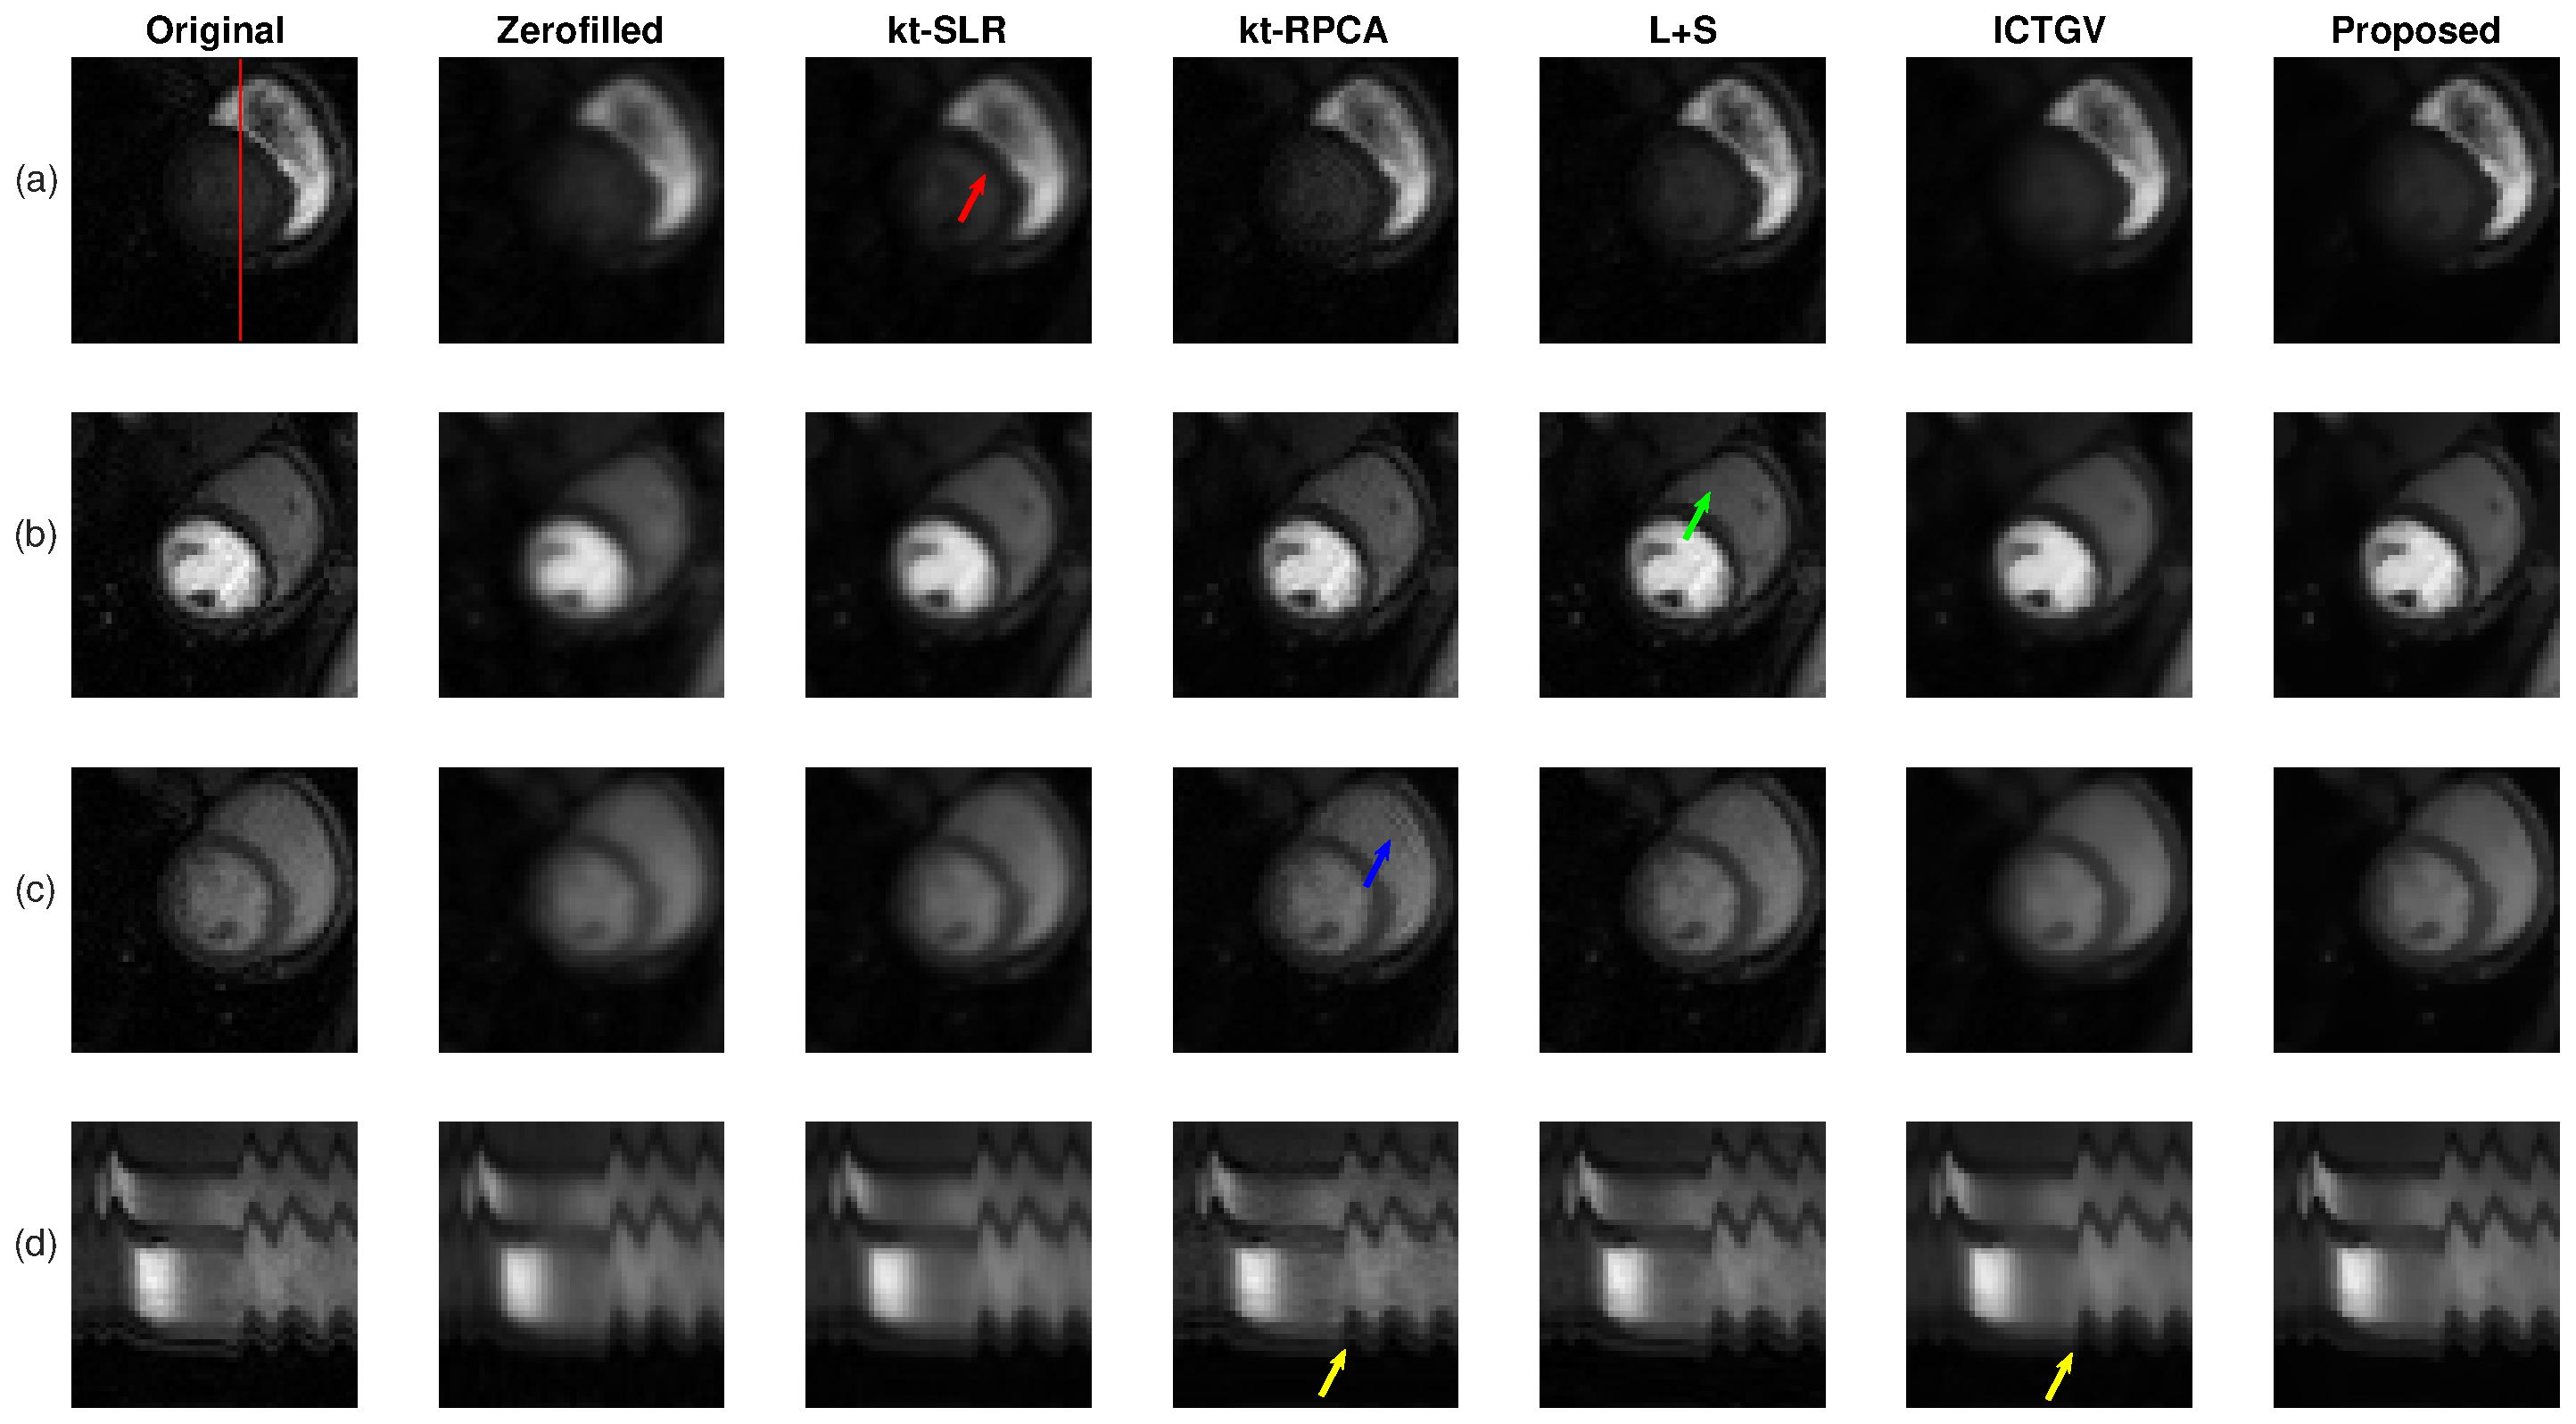
\includegraphics[width=1\textwidth]{img/tgvnn/figure4_perfusion_frames.eps}
\caption{各个模型在cardiac数据上的重建结果(时间方向)。(a)、(b)和(c)行分别为重建图像的第11,第21和第54帧;(d)行是通过心脏的一列(红线)在时间序列图像。}
\label{fig:perfusion_frames}
\end{figure}

图\ref{fig:breast1},\ref{fig:breast2}和\ref{fig:breast3}分别展示了各个模型在Breast1(第105帧),Breast2(第25帧)和Breast3(第1帧)上的重建结果。本文的模型不仅取得了最高的SER和SSIM,也可以很好地抑制空间伪影(蓝色箭头)并重建肿瘤区域(红色箭头)。kt-SLR,kt-RPCA和ICTGV并不适用于胸部DCE-MRI数据集。有趣的是,L+S在重建肿瘤方面的表现从视觉上看略优于本文的模型,但是L+S重建图像的SER和SSIM均很低,并且背景区域有残留的空间伪影(蓝色箭头)。

\begin{figure}
\centering
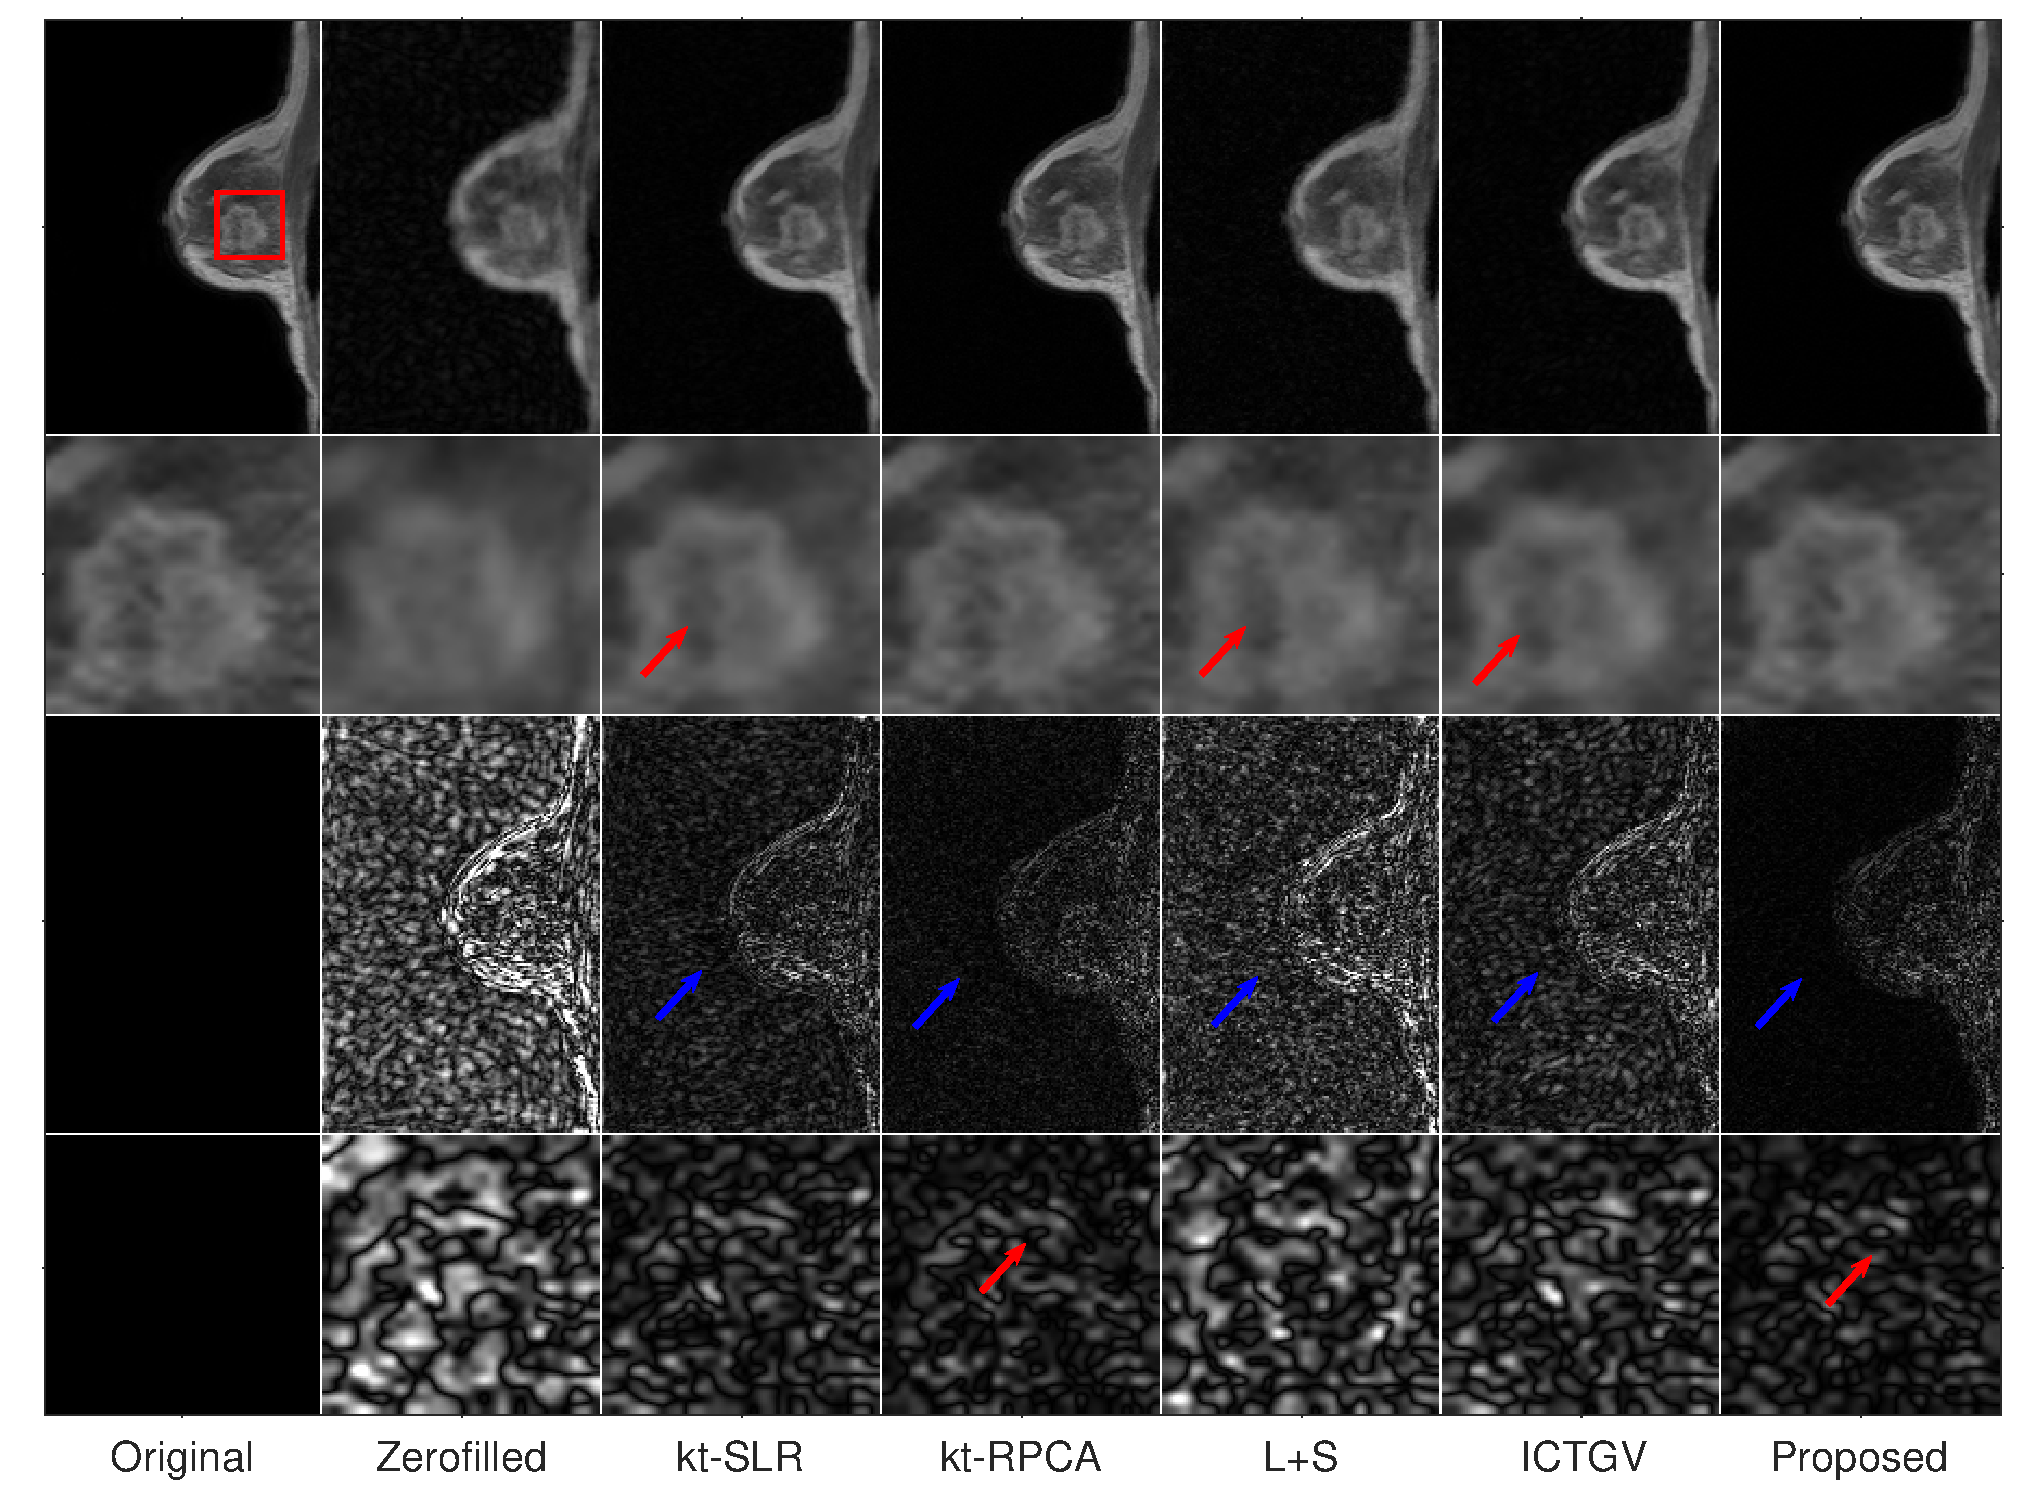
\includegraphics[width=1\textwidth]{img/tgvnn/figure5_breast1.eps}
\caption{各个模型在Breast1上的重建结果(第105帧)。为了在视觉上更好地展示胸部肿瘤,我们切除了心脏部分。第1行:重建图像;第2行:红色方框区域的放大图像;第3行:相对于原始图像的差值图像;第4行:红色方框区域放大的差值图像。为了增加可见度,差值图像放大了10倍。}
\label{fig:breast1}
\end{figure} 

\begin{figure}
\centering
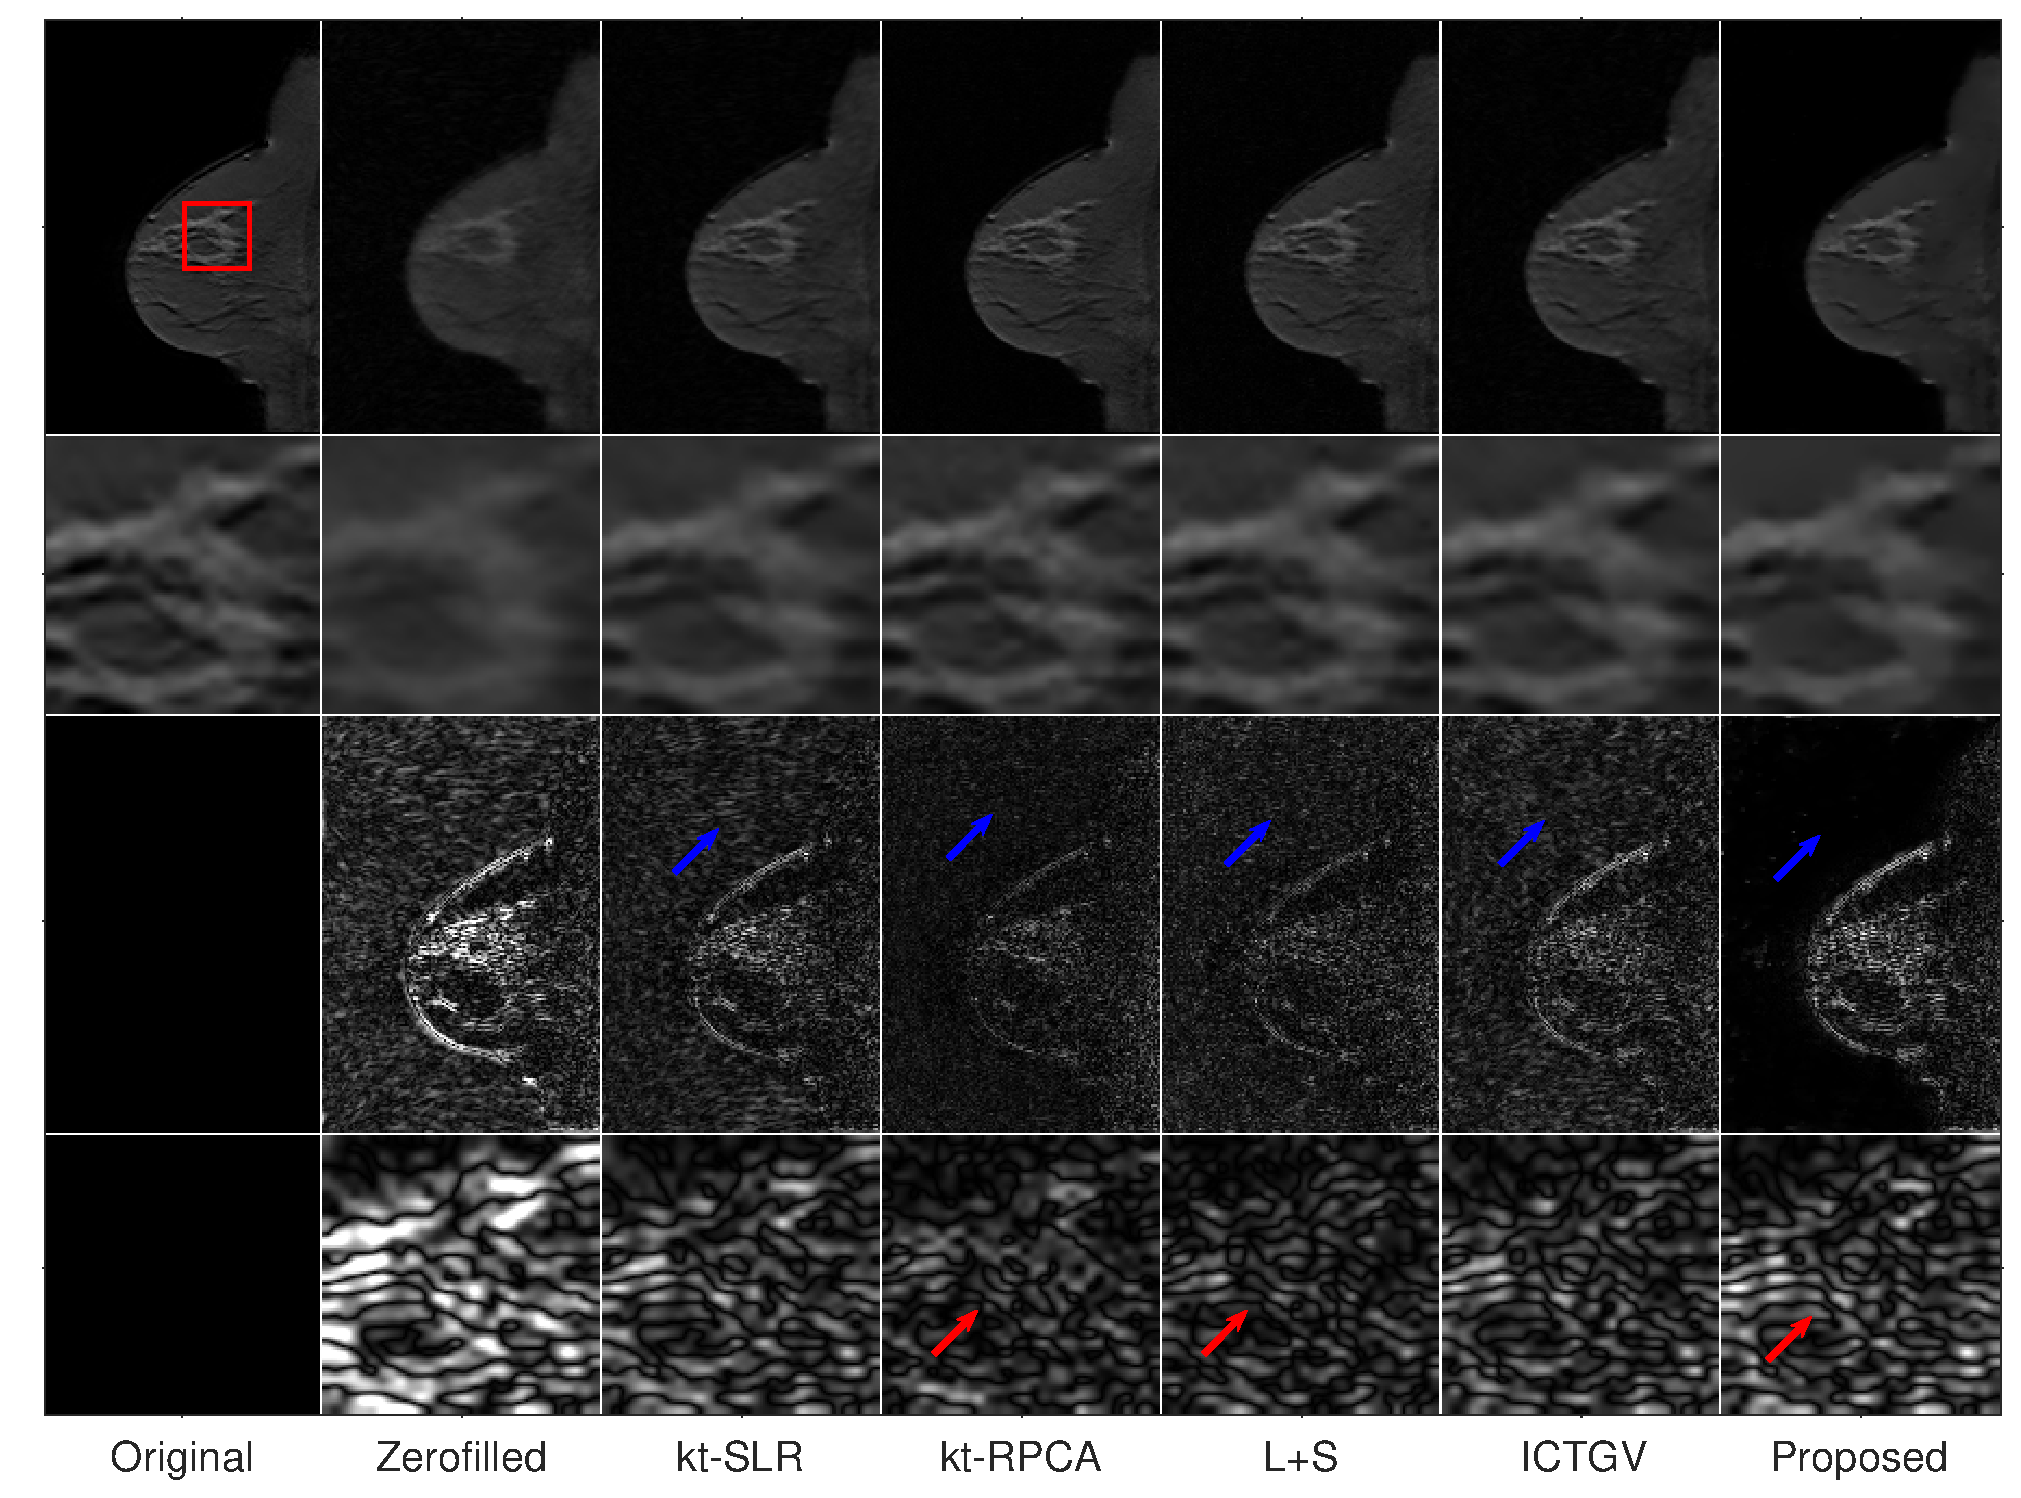
\includegraphics[width=1\textwidth]{img/tgvnn/breast2.eps}
\caption{各个模型在Breast2上的重建结果(第25帧)。为了在视觉上更好地展示胸部肿瘤,我们切除了心脏部分。第1行:重建图像;第2行:红色方框区域的放大图像;第3行:相对于原始图像的差值图像;第4行:红色方框区域放大的差值图像。为了增加可见度,差值图像放大了10倍。}
\label{fig:breast2}
\end{figure} 

\begin{figure}
\centering
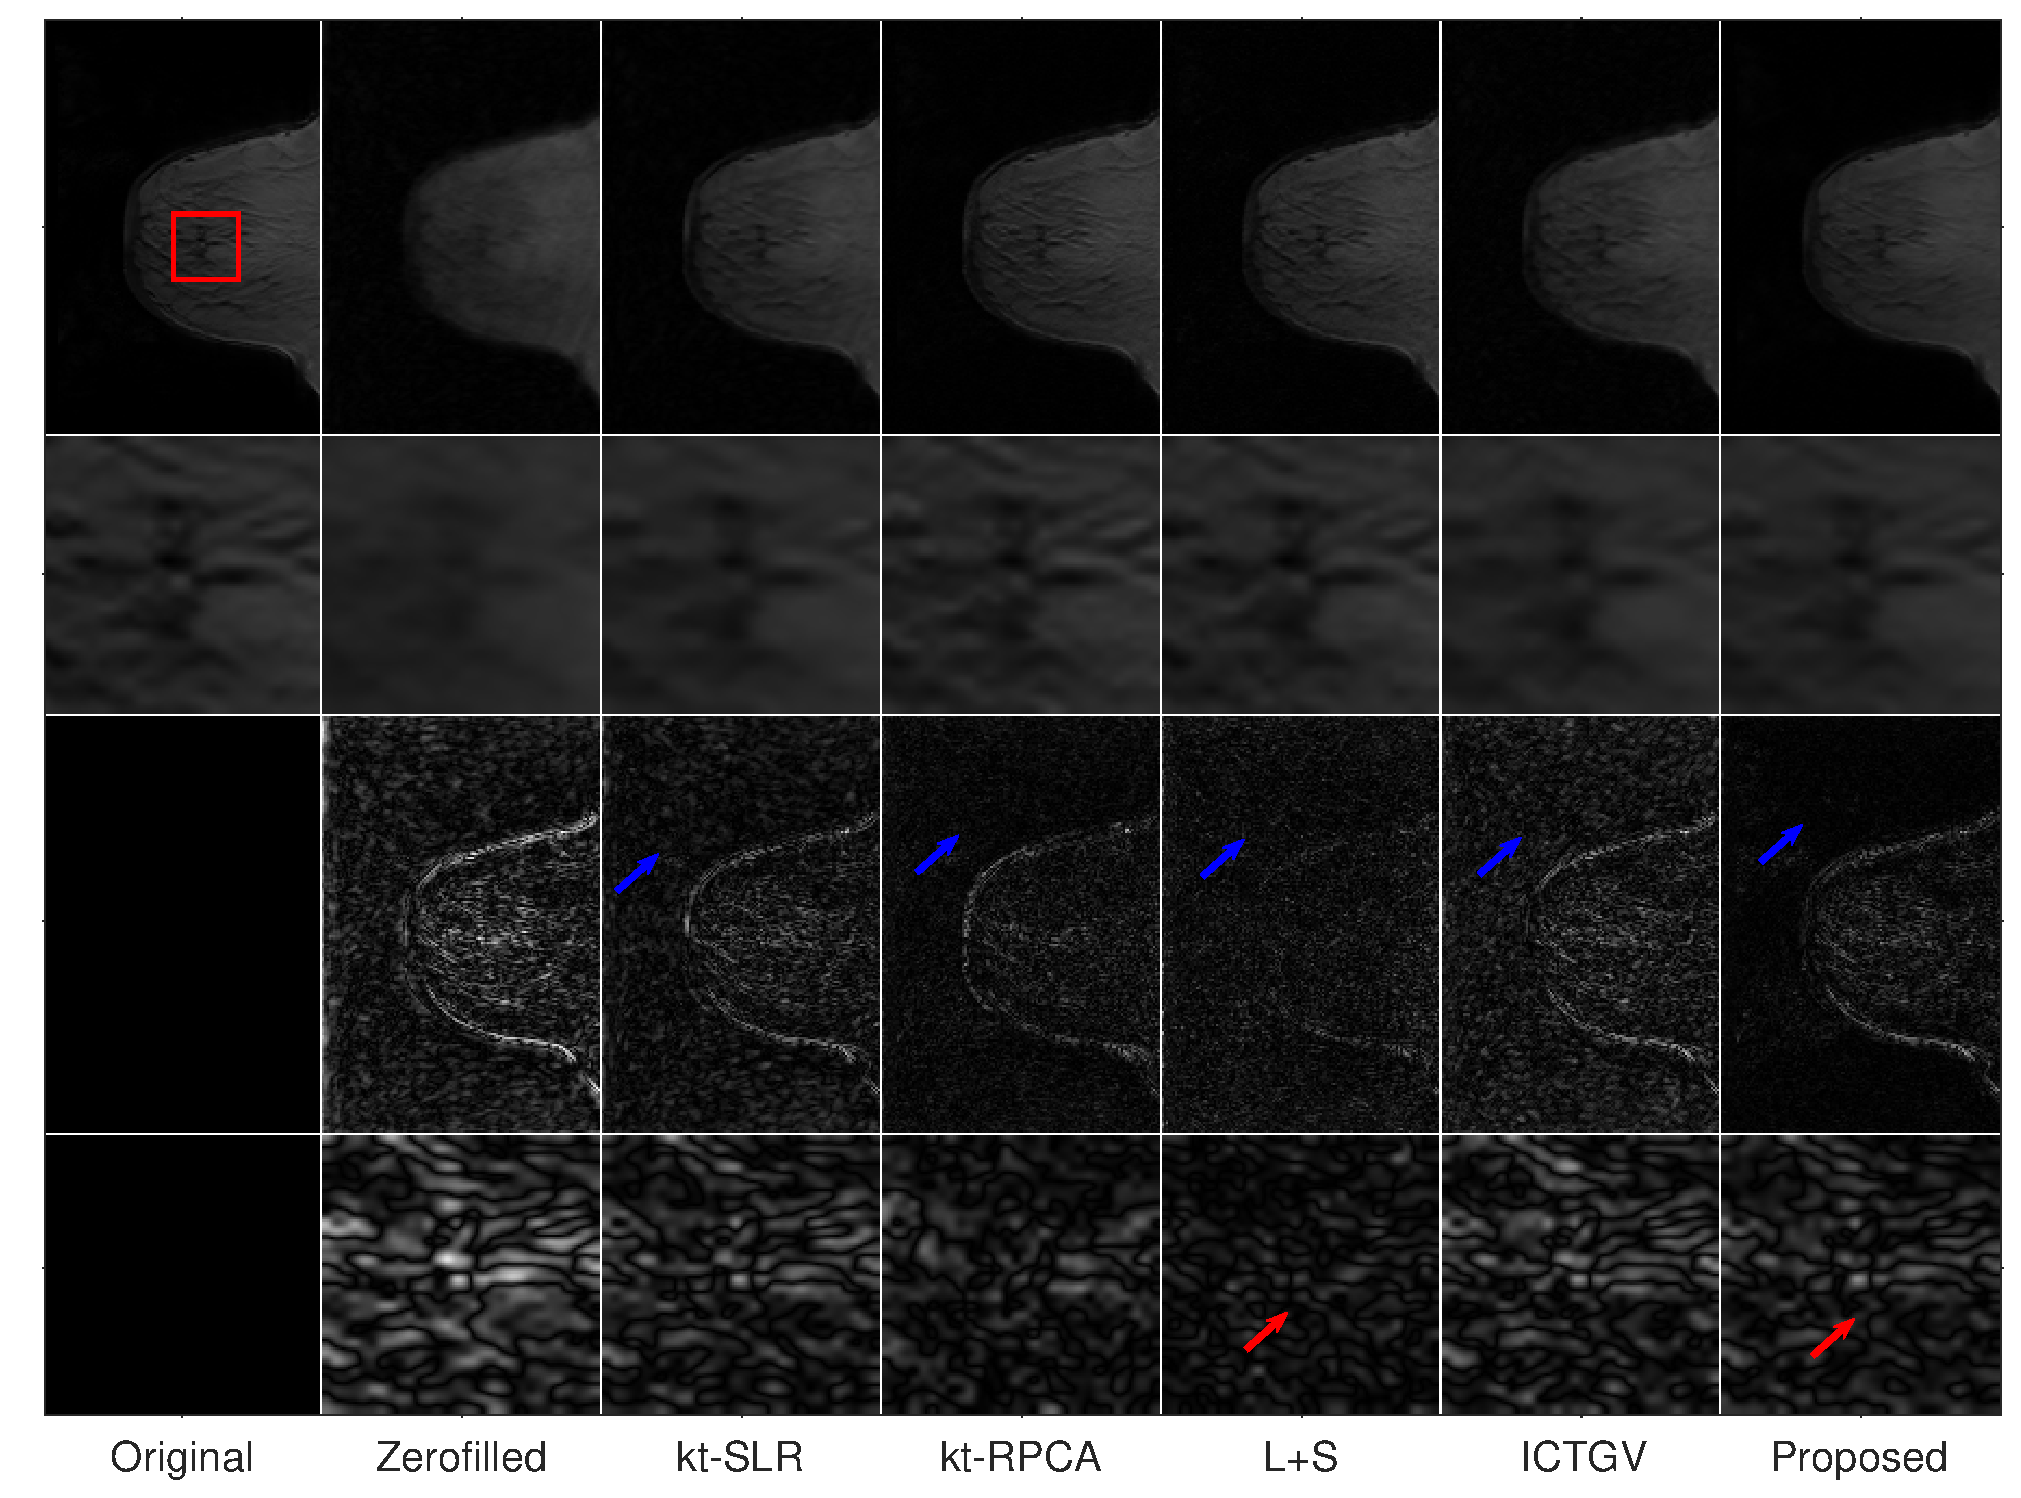
\includegraphics[width=1\textwidth]{img/tgvnn/breast3.eps}
\caption{各个模型在Breast3上的重建结果(第1帧)。为了在视觉上更好地展示胸部肿瘤,我们切除了心脏部分。第1行:重建图像;第2行:红色方框区域的放大图像;第3行:相对于原始图像的差值图像;第4行:红色方框区域放大的差值图像。为了增加可见度,差值图像放大了10倍。}
\label{fig:breast3}
\end{figure} 

我们也比较了各个模型在Breast1数据上的运行时间,如表\ref{tab:time3}所示。值得注意的是ICTGV也有GPU版本的代码,但在安装的时候出现了问题,导致程序无法在我们的工作站上运行,因此这里只展示了ICTGV在CPU上的运行时间。可以看出,kt-SLR和kt-RPCA的运行速度相对较快,这是因为它们只包含时间方向上的稀疏项。虽然本文模型的MATLAB代码运行速度较慢(2812.90 s),但GPU版本的运行时间只需要28.35 s,GPU的使用使得程序运行速度提高了将近100倍。
\begin{table}
\centering
\caption{各个模型在Breast1数据上运行时间比较}
\begin{center}
\begin{tabular}{|l|l|l|l|l|l|l|}
\hline
\hline
\multirow{2}{*}{模型} & kt-SLR & kt-RPCA & L+S & ICTGV & Proposed & Proposed \\
& (CPU) & (CPU) & (CPU) & (CPU) & (CPU) & (GPU) \\
\hline
时间 (s) & 5794.88 & 641.71 & 493.80 & 2572.04 & 2812.90 & 28.35 \\
\hline
\end{tabular}
\end{center}
\label{tab:time3}
\end{table}

为了展示胸部肿瘤随时间的变化,我们也绘制了Breast1肿瘤区域的平均像素值时间曲线,如图\ref{fig:breast1_time}所示。平均像素值时间曲线是指肿瘤区域(红色方框)的平均像素值随时间变化的曲线,是胸部图像肿瘤区域重建效果的常用评估方法之一。可以看到,本文的模型在造影剂注入之前和之后都可以很好地拟合曲线,并且方差较低。相反的,kt-SLR和kt-RPCA拟合曲线的方差很高,尤其在注入造影剂之后(蓝色箭头)。黄色箭头表明kt-RPCA不能很好地拟合前10—-15帧。L+S最后5帧的拟合效果很差,这一点从绿色箭头中可以更容易看出。
\begin{figure}
\centering
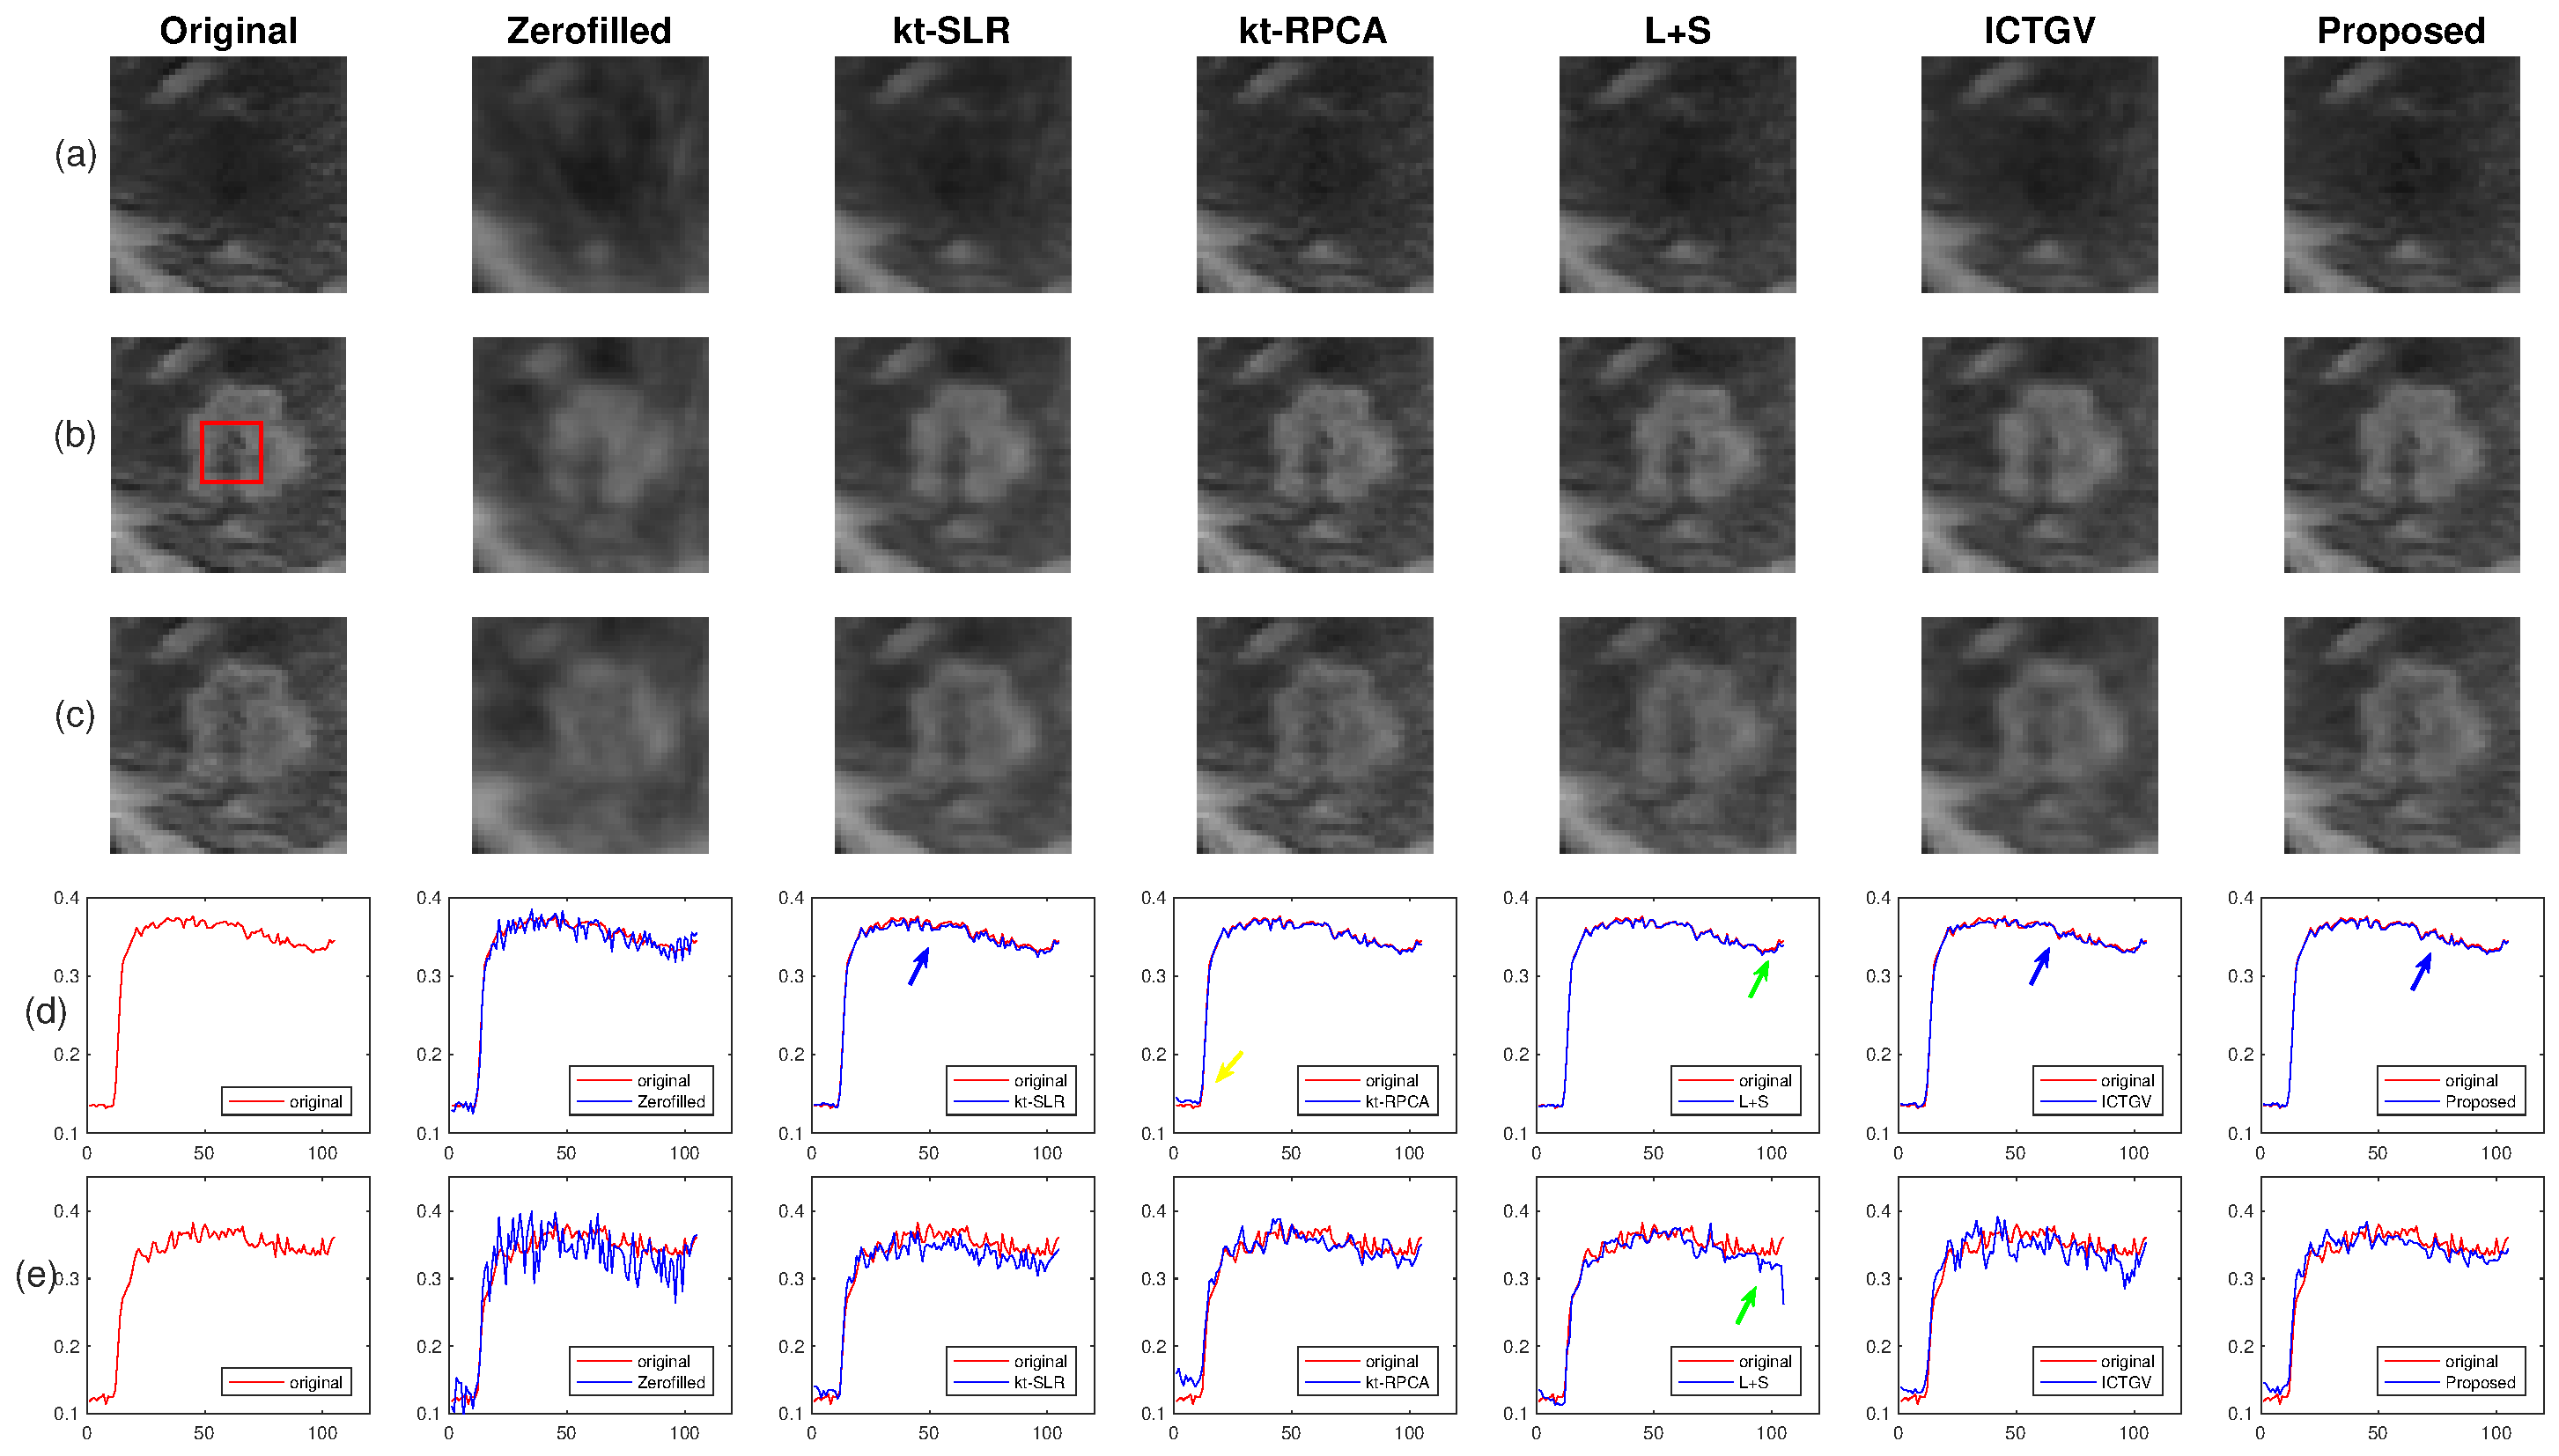
\includegraphics[width=1\textwidth]{img/tgvnn/figure6_breast1_frames.eps}
\caption{各个模型在Breast1上的重建结果(时间方向)。(a)、(b)和(c)行分别为重建图像的第1,第53和第105帧;(d)行是肿瘤区域(红色方框)的平均像素值时间曲线;(e)行是肿瘤区域某一像素点的像素值时间曲线。}
\label{fig:breast1_time}
\end{figure} 

为了测试各个模型在不同加速因子下的表现,我们选择了5个不同数量的采样线,即12、22、32、42和52,相应的加速因子分别为17.0、9.5、6.6、5.1和4.2。表\ref{tab:sampling}展示了不同模型在不同加速因子下在Breast1数据上的表现。可以看出,本文的模型在不同的加速因子下都可以得到最高的SER和SSIM,这表明了本文模型的一致性。
\begin{table}
	\centering
	\caption{各个模型在不同加速因子下在Breast1数据上的重建结果}
	\begin{tabular}{|c|c|c|c|c|c|c|}
		\hline
		\hline
		\multicolumn{2}{|c|}{\diagbox{模型}{采样线}} & 12 & 22 & 32 & 42 & 52\\	
		\hline
		\multirow{2}{*}{Zerofilled}
		&SER & 5.98 & 9.06 & 11.32 & 12.93 & 14.33 \\
		\cline{2-7}&SSIM & 0.3218 & 0.4108 & 0.4820 & 0.5350 & 0.5818 \\
		\hline
		\multirow{2}{*}{kt-SLR}
		&SER & 15.16 & 16.10 & 17.42 & 19.07 & 19.11 \\
		\cline{2-7}&SSIM & 0.7323 & 0.7312 & 0.7712 & 0.8087 & 0.7989 \\
		\hline
		\multirow{2}{*}{kt-RPCA}
		&SER & 13.10 & 17.74 & 19.31 & 20.26 & 21.13 \\
		\cline{2-7}&SSIM & 0.6241 & 0.8356 & 0.8857 & 0.9061 & 0.9245 \\
		\hline
		\multirow{2}{*}{L+S}
		&SER & 12.75 & 16.00 & 17.60 & 18.73 & 19.64 \\
		\cline{2-7}&SSIM & 0.5885 & 0.7119 & 0.7675 & 0.8018 & 0.8275 \\
		\hline
		\multirow{2}{*}{ICTGV}
		&SER & 13.56 & 15.30 & 16.31 & 17.03 & 17.56 \\
		\cline{2-7}&SSIM & 0.6001 & 0.6485 & 0.6735 & 0.6895 & 0.7007\\
		\hline
		\multirow{2}{*}{Proposed}
		&SER & \textbf{16.49} & \textbf{19.06} & \textbf{20.56} & \textbf{21.82} & \textbf{22.96}\\
		\cline{2-7}&SSIM & \textbf{0.8620} & \textbf{0.9119} & \textbf{0.9402} & \textbf{0.9535} & \textbf{0.9632}\\
		\hline
	\end{tabular}
	\label{tab:sampling}
\end{table}

为了评估本文模型在不同采样模式下的表现,我们也比较了各个模型在Cartesian采样模式下(如图\ref{fig:mask3}(b))的重建结果。表\ref{tab:cartesian}展示了各个模型在Cartesian采样模式下在Breast1数据上的重建结果。可以看出,本文的模型和L+S都得到了最高的SER(28.46),而且本文模型得到了最高的SSIM。其他的模型在Cartesian采样模式下的表现不理想。
\begin{table}
\centering
\caption{各个模型在Cartesian采样模式下在Breast1数据上的重建结果}
\begin{center}
\begin{tabular}{|l|l|l|l|l|l|l|}
\hline
\hline
模型 & Zerofilled & kt-SLR & kt-RPCA & L+S & ICTGV & Proposed \\
\hline
SER & 11.29 & 16.60 & 16.86 & 14.55 & 14.33 & \textbf{17.79} \\
\hline
SSIM & 0.7370 & 0.8942 & 0.9126 & 0.8379 & 0.7681 & \textbf{0.9169}\\
\hline
\end{tabular}
\end{center}
\label{tab:cartesian}
\end{table}

\section{本章小结}
在本章中,我们回顾了动态MR压缩感知的经典模型,并基于图像分解思想提出了利用二阶时空TGV泛函和核范数的重建模型。其中,核范数用来建模时间高度相关的背景部分,可以很好地消除空间伪影;二阶时空TGV泛函可以刻画图像中的光滑部分,在保持图像边缘的同时可以抑制阶梯效应的产生。我们使用Primal-Dual算法来求解模型,并并给出了算法收敛时的范数估计。我们也利用了GPU来加速MATLAB程序。在PINCAT、心脏灌注和胸部DCE-MRI数据上的实验表明,在不同的采样模式和加速因子下,本文的模型都比最前沿的模型在消除空间伪影、保持边缘上的表现更好,尤其是在胸部DCE-MRI数据上。

实验中,我们在PINCAT数据上手动调试了参数,然后将这组参数应用到其他数据中。这样的调参方法需要满足一个假设,即这组参数可以推广到其他数据中。但是在实际中,并不是所有的模型都满足这样的假设。这些模型的参数可能仅仅取决于噪声水平、加速因子等。因此本章中所展示的结果有一定的局限性,对于某个模型和某组数据而言,不同的参数可能会有更好的结果。

















